\documentclass[11pt,a4paper]{report}
\usepackage[utf8]{inputenc}
\usepackage[spanish]{babel}
\usepackage{geometry}
\geometry{top=2.0cm,bottom=2.0cm,left=2.5cm,right=2.5cm}
\usepackage{fancyhdr}
\usepackage{graphicx}
\graphicspath{{../04 Mapas/}}
\usepackage{amsmath,amssymb}
\usepackage{booktabs}
\usepackage{tabularx}
\usepackage{xcolor}
\usepackage{float}
\usepackage{titlesec}
\usepackage{setspace}

\definecolor{navyblue}{RGB}{31,78,121}
\definecolor{darkslate}{RGB}{47,85,151}

\titleformat{\chapter}[display]
  {\normalfont\bfseries\color{navyblue}}
  {\filleft\Huge\textbf{\chaptertitlename\ \thechapter}}
  {1ex}
  {\titlerule\vspace{1ex}\LARGE}
  [\vspace{1ex}\titlerule]

\titleformat{\section}
  {\normalfont\Large\bfseries\color{navyblue}}
  {\thesection}{1em}{}

\pagestyle{fancy}
\fancyhf{}
\rhead{\small\textcolor{darkslate}{Anexo A: Cartografía y Planos de Gran Formato}}
\lhead{\small\textcolor{darkslate}{MCH Río Blanco 100 kW - Puno}}
\rfoot{\small Página \thepage}
\lfoot{\small UNAP - FIME / Consultoría RER}

\begin{document}

\begin{titlepage}
\begin{center}
    \vspace*{2cm}
    {\Large\bfseries UNIVERSIDAD NACIONAL DEL ALTIPLANO PUNO}\\[0.5em]
    {\large FACULTAD DE INGENIERÍA MECÁNICA ELÉCTRICA}\\[2.5cm]

    \rule{\linewidth}{2pt}\\[0.4cm]
    {\huge\bfseries\color{navyblue} ANEXO A: CARTOGRAFÍA SATELITAL, RED GEODÉSICA Y PLANOS DE INGENIERÍA DE DETALLE}\\[0.4cm]
    {\Large\bfseries PROYECTO MICROCENTRAL HIDROELÉCTRICA RÍO BLANCO 100 kW}\\[0.4cm]
    {\large Distrito de Ollachea, Provincia de Carabaya, Departamento de Puno}\\[0.4cm]
    \rule{\linewidth}{2pt}\\[2.5cm]

    \textbf{Contenido del Expediente:}\\
    Láminas Cartográficas Satelitales ESRI HD (Escala 1:1,000 a 1:1,000,000)\\
    Red Geodésica de Control Horizontal y Vertical de Orden ``C'' (IGN)\\
    Planos Estructurales, Hidráulicos y Diagramas Eléctricos Unifilares\\[2cm]

    \vfill
    {\large Puno -- Perú}\\[0.3em]
    {\normalsize Setiembre 2024 / 2026}
\end{center}
\end{titlepage}

\chapter{Memoria Descriptiva Cartográfica y Geodésica}
\section{Marco Geodésico y Proyección Cartográfica}
El presente anexo reúne cartografía digital y planos conceptuales del caso de prefactibilidad. No es cartografía oficial ni levantamiento certificado por el IGN. Las coordenadas, escalas, límites, trazados y capas requieren contraste con cartografía oficial y verificación de campo antes de replanteo o diseño.
\begin{itemize}
    \item \textbf{Elipsoide de Referencia:} WGS-84 (World Geodetic System 1984 / GRS80).
    \item \textbf{Proyección Cartográfica:} Universal Transversa de Mercator (UTM), Zona 19 Sur.
    \item \textbf{Meridiano Central:} $69^\circ\text{ Oeste}$ ($k_0 = 0.999600$).
    \item \textbf{Modelo Geoidal:} EGM2008 (Ondulación Geoidal $N = +38.45\text{ m}$).
    \item \textbf{Factor de Escala Combinado ($K$):} $0.999234$.
    \item \textbf{Convergencia de Meridianos:} $\gamma = -0^\circ 34' 12.8''$.
\end{itemize}

\section{Índice de láminas conceptuales de prefactibilidad}
\begin{table}[H]
\centering
\small
\begin{tabularx}{\linewidth}{llcX}
\toprule
\textbf{Código} & \textbf{Título Oficial de la Lámina} & \textbf{Escala} & \textbf{Descripción del Contenido} \\
\midrule
LAM-01 & Ubicación Regional y Acceso Vial & 1 : 1,000,000 & Imagen satelital real de Puno, Macusani, Ollachea y PE-34B. \\
LAM-02 & Modelo Digital de Elevación y Cuenca & 1 : 25,000 & DEM 3D con curvas cada 25m y red hidrográfica Strahler. \\
LAM-03 & Ortofoto y Trazado de Obras Civiles & 1 : 2,500 & Ortofoto satelital ESRI HD con trazo de bocatoma a restitución. \\
LAM-04 & Isoyetas de Precipitación SENAMHI & 1 : 100,000 & Distribución espacial de lluvias medias anuales (1994-2023). \\
LAM-05 & Perfil Longitudinal y Golpe de Ariete & 1 : 1,500 & Perfil de tubería forzada, sobrepresión y 4 dados de anclaje. \\
LAM-06 & Referencias topográficas conceptuales & Escala referencial & Puntos por verificar en levantamiento de campo. \\
LAM-07 & Geología y Riesgos de Ladera & 1 : 2,500 & Litología Formación Sandia, fallas y estabilidad de taludes. \\
LAM-08 & Zonificación de Usos Productivos & 1 : 5,000 & Red MT 10 kV, centros agroindustriales y poblado Ollachea. \\
PL-01 & Bocatoma Tirolesa y Desarenador & 1 : 50 & Azud ciclópeo, rejilla Coanda 20° y 2 naves con vertedero Sutro. \\
PL-02 & Cámara de Carga y Aliviadero & 1 : 50 & Tanque de 22.5 m³, sumergencia hs=1.40m y aliviadero. \\
PL-03 & Casa de Máquinas y Grupo Pelton & 1 : 50 & Planta casa de máquinas, turbina 2 inyectores y alternador. \\
PL-04 & Diagrama Unifilar y Subestación & 1 : 100 & Esquema unifilar 125 kVA 0.38/10 kV, relés ANSI y tierra IEEE 80. \\
\bottomrule
\end{tabularx}
\caption{Índice General de Láminas Cartográficas y Planos de Ingeniería de Detalle.}
\label{tab:catalogo_laminas}
\end{table}

\chapter{Láminas Cartográficas Satelitales y Geodésicas}

\begin{figure}[H]
\centering
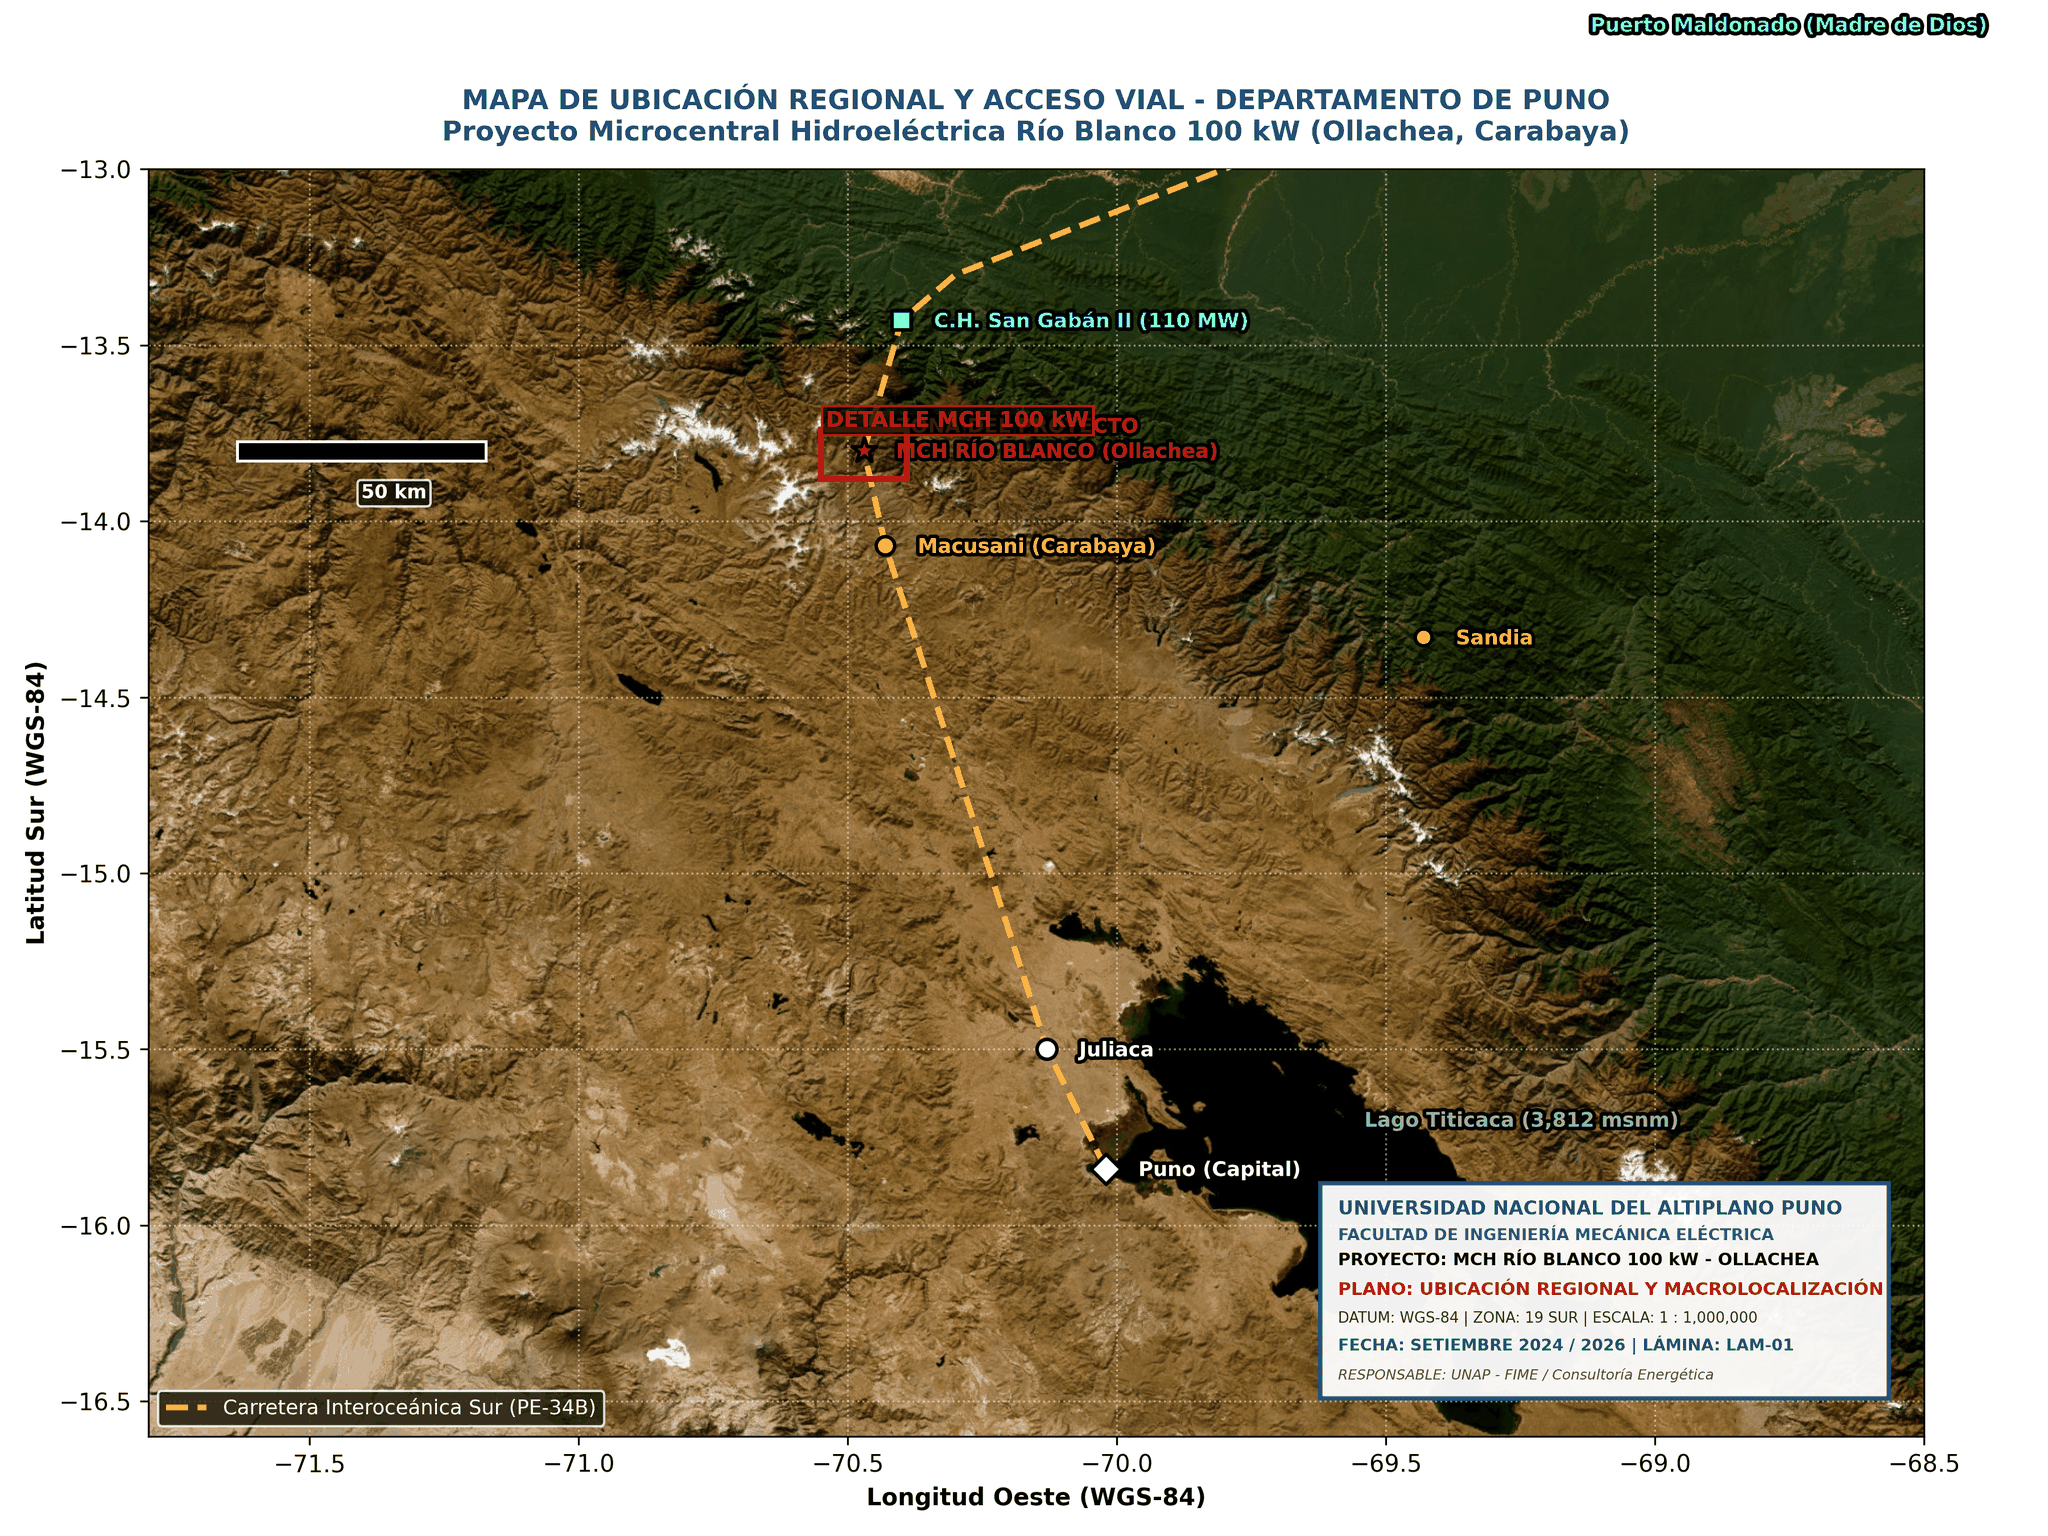
\includegraphics[width=\linewidth]{Mapa_01_Ubicacion_Regional_Puno.png}
\caption{LÁMINA LAM-01: Mapa de Ubicación Regional y Acceso Vial sobre Imagen Satelital Real.}
\end{figure}

\begin{figure}[H]
\centering
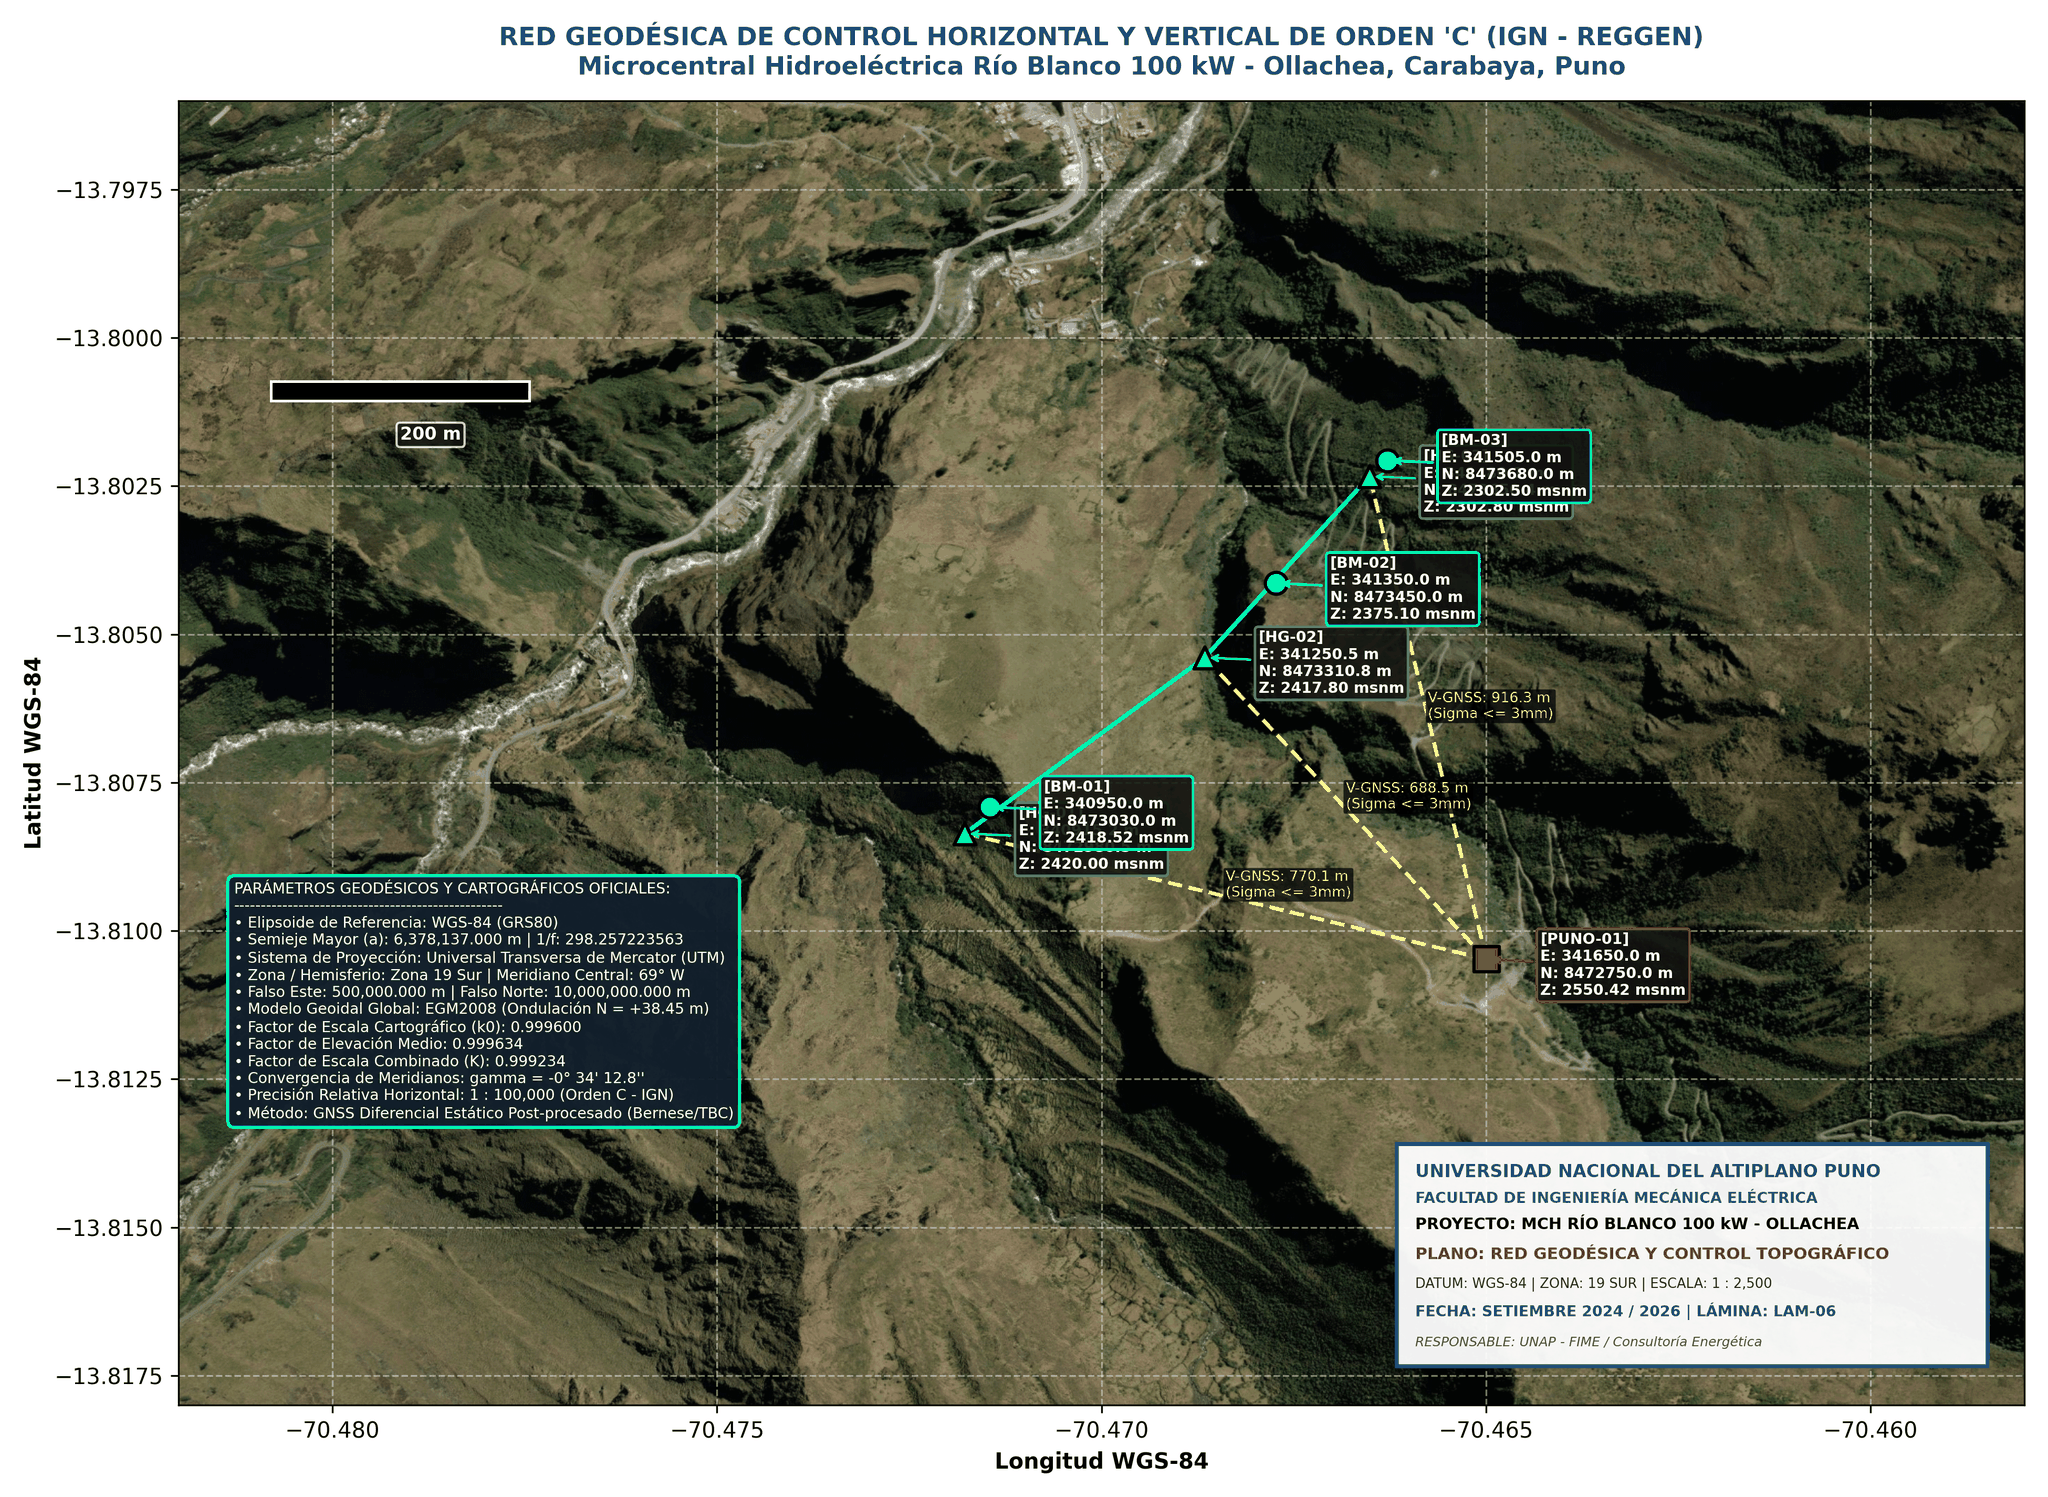
\includegraphics[width=\linewidth]{Mapa_06_Red_Control_Geodesico_IGN.png}
\caption{LÁMINA LAM-06: Red Geodésica de Control Horizontal y Vertical de Orden ``C'' (IGN - REGGEN).}
\end{figure}

\begin{figure}[H]
\centering
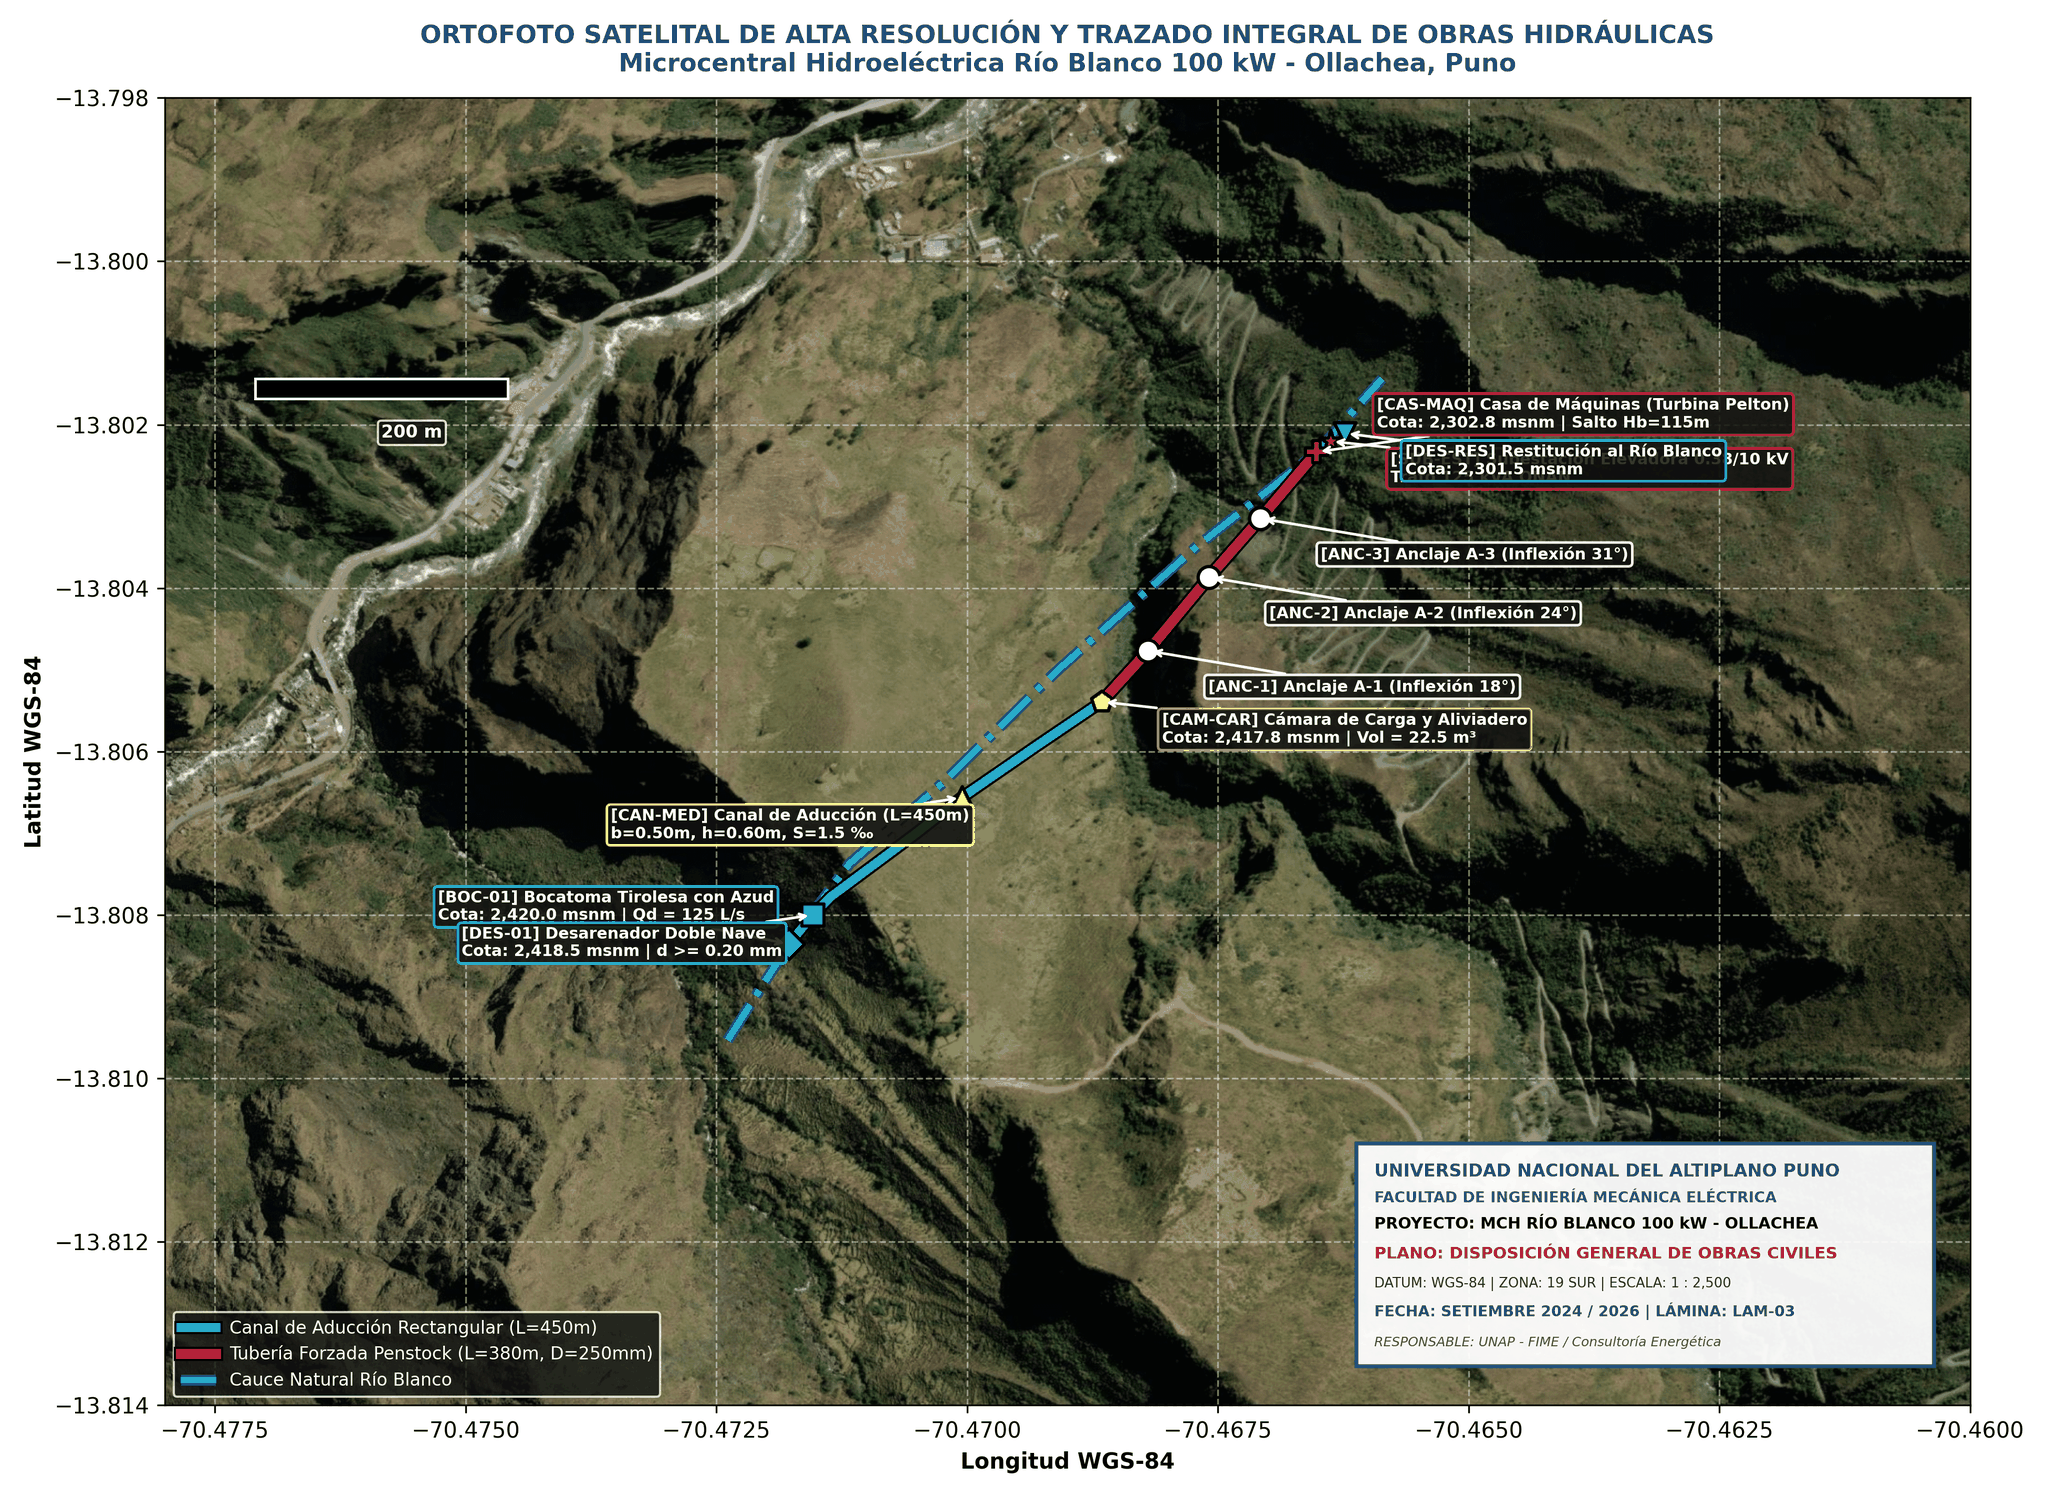
\includegraphics[width=\linewidth]{Mapa_03_Esquema_Obras_Hidraulicas_Trazo.png}
\caption{LÁMINA LAM-03: Ortofoto Satelital de Alta Resolución con Trazado de Obras Hidráulicas.}
\end{figure}

\begin{figure}[H]
\centering
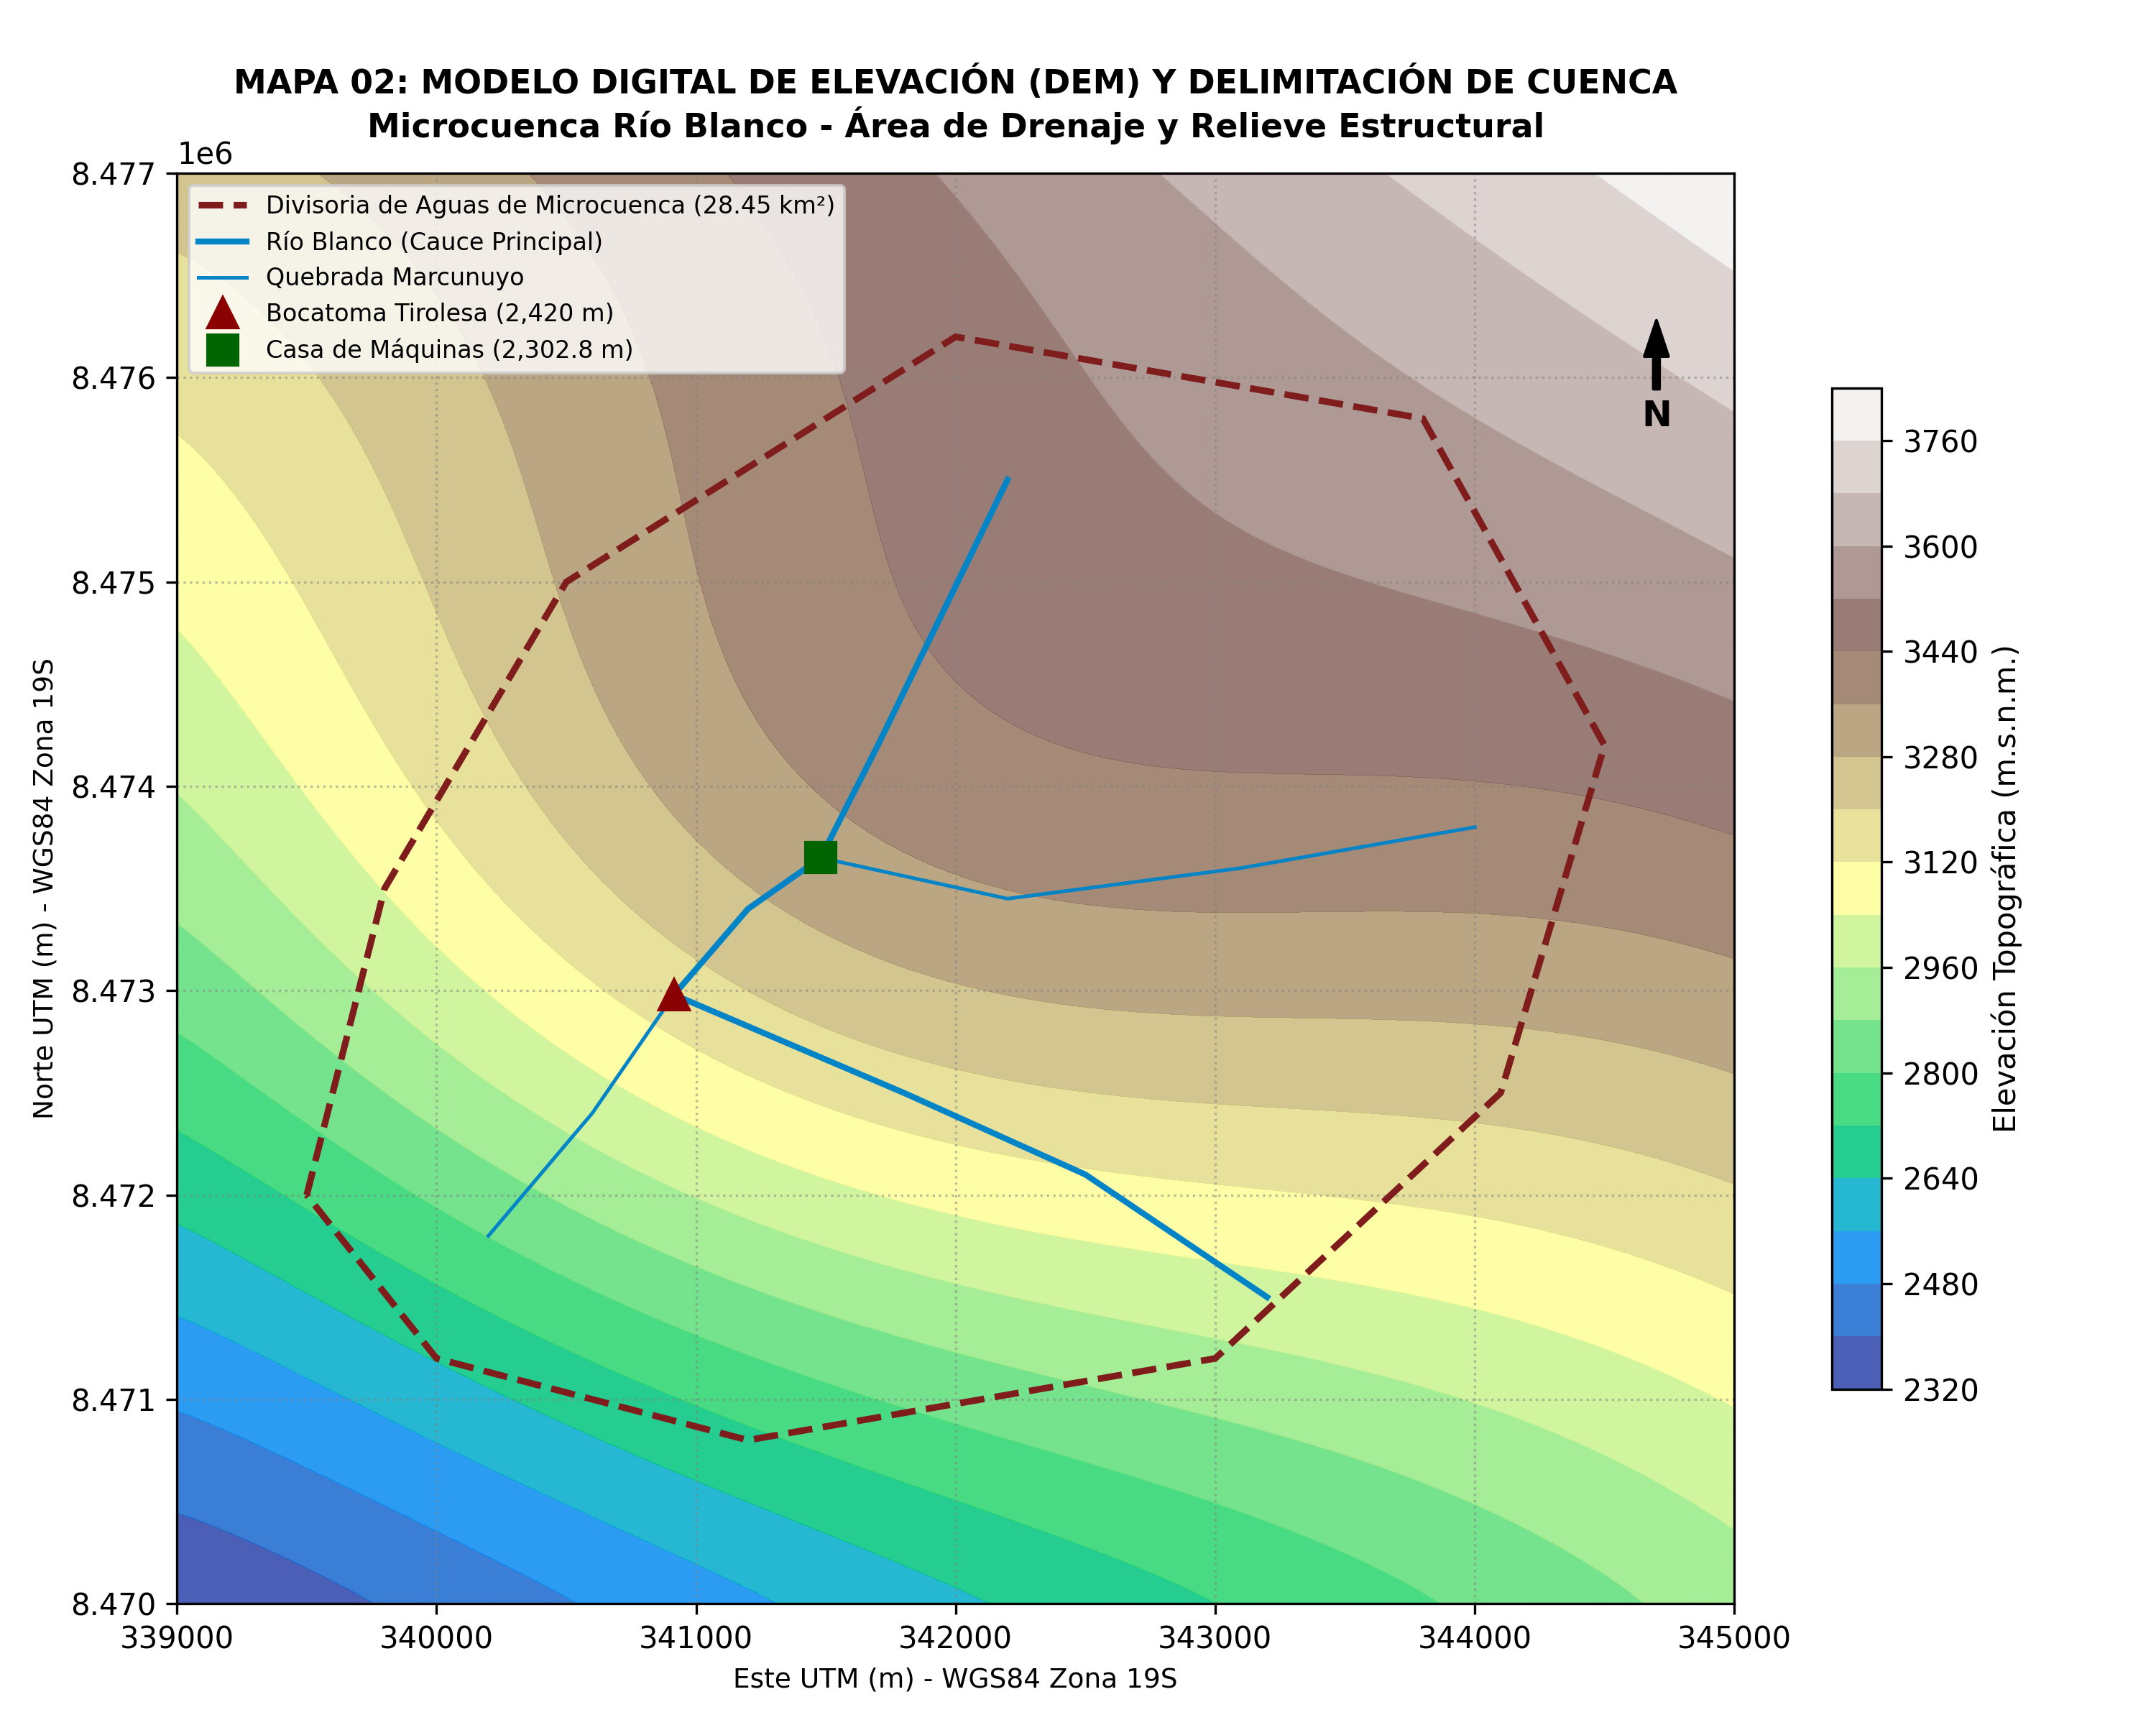
\includegraphics[width=\linewidth]{Mapa_02_Topografia_DEM_y_Cuenca.png}
\caption{LÁMINA LAM-02: Modelo Digital de Elevación (DEM 3D) y Delimitación de Microcuenca.}
\end{figure}

\begin{figure}[H]
\centering
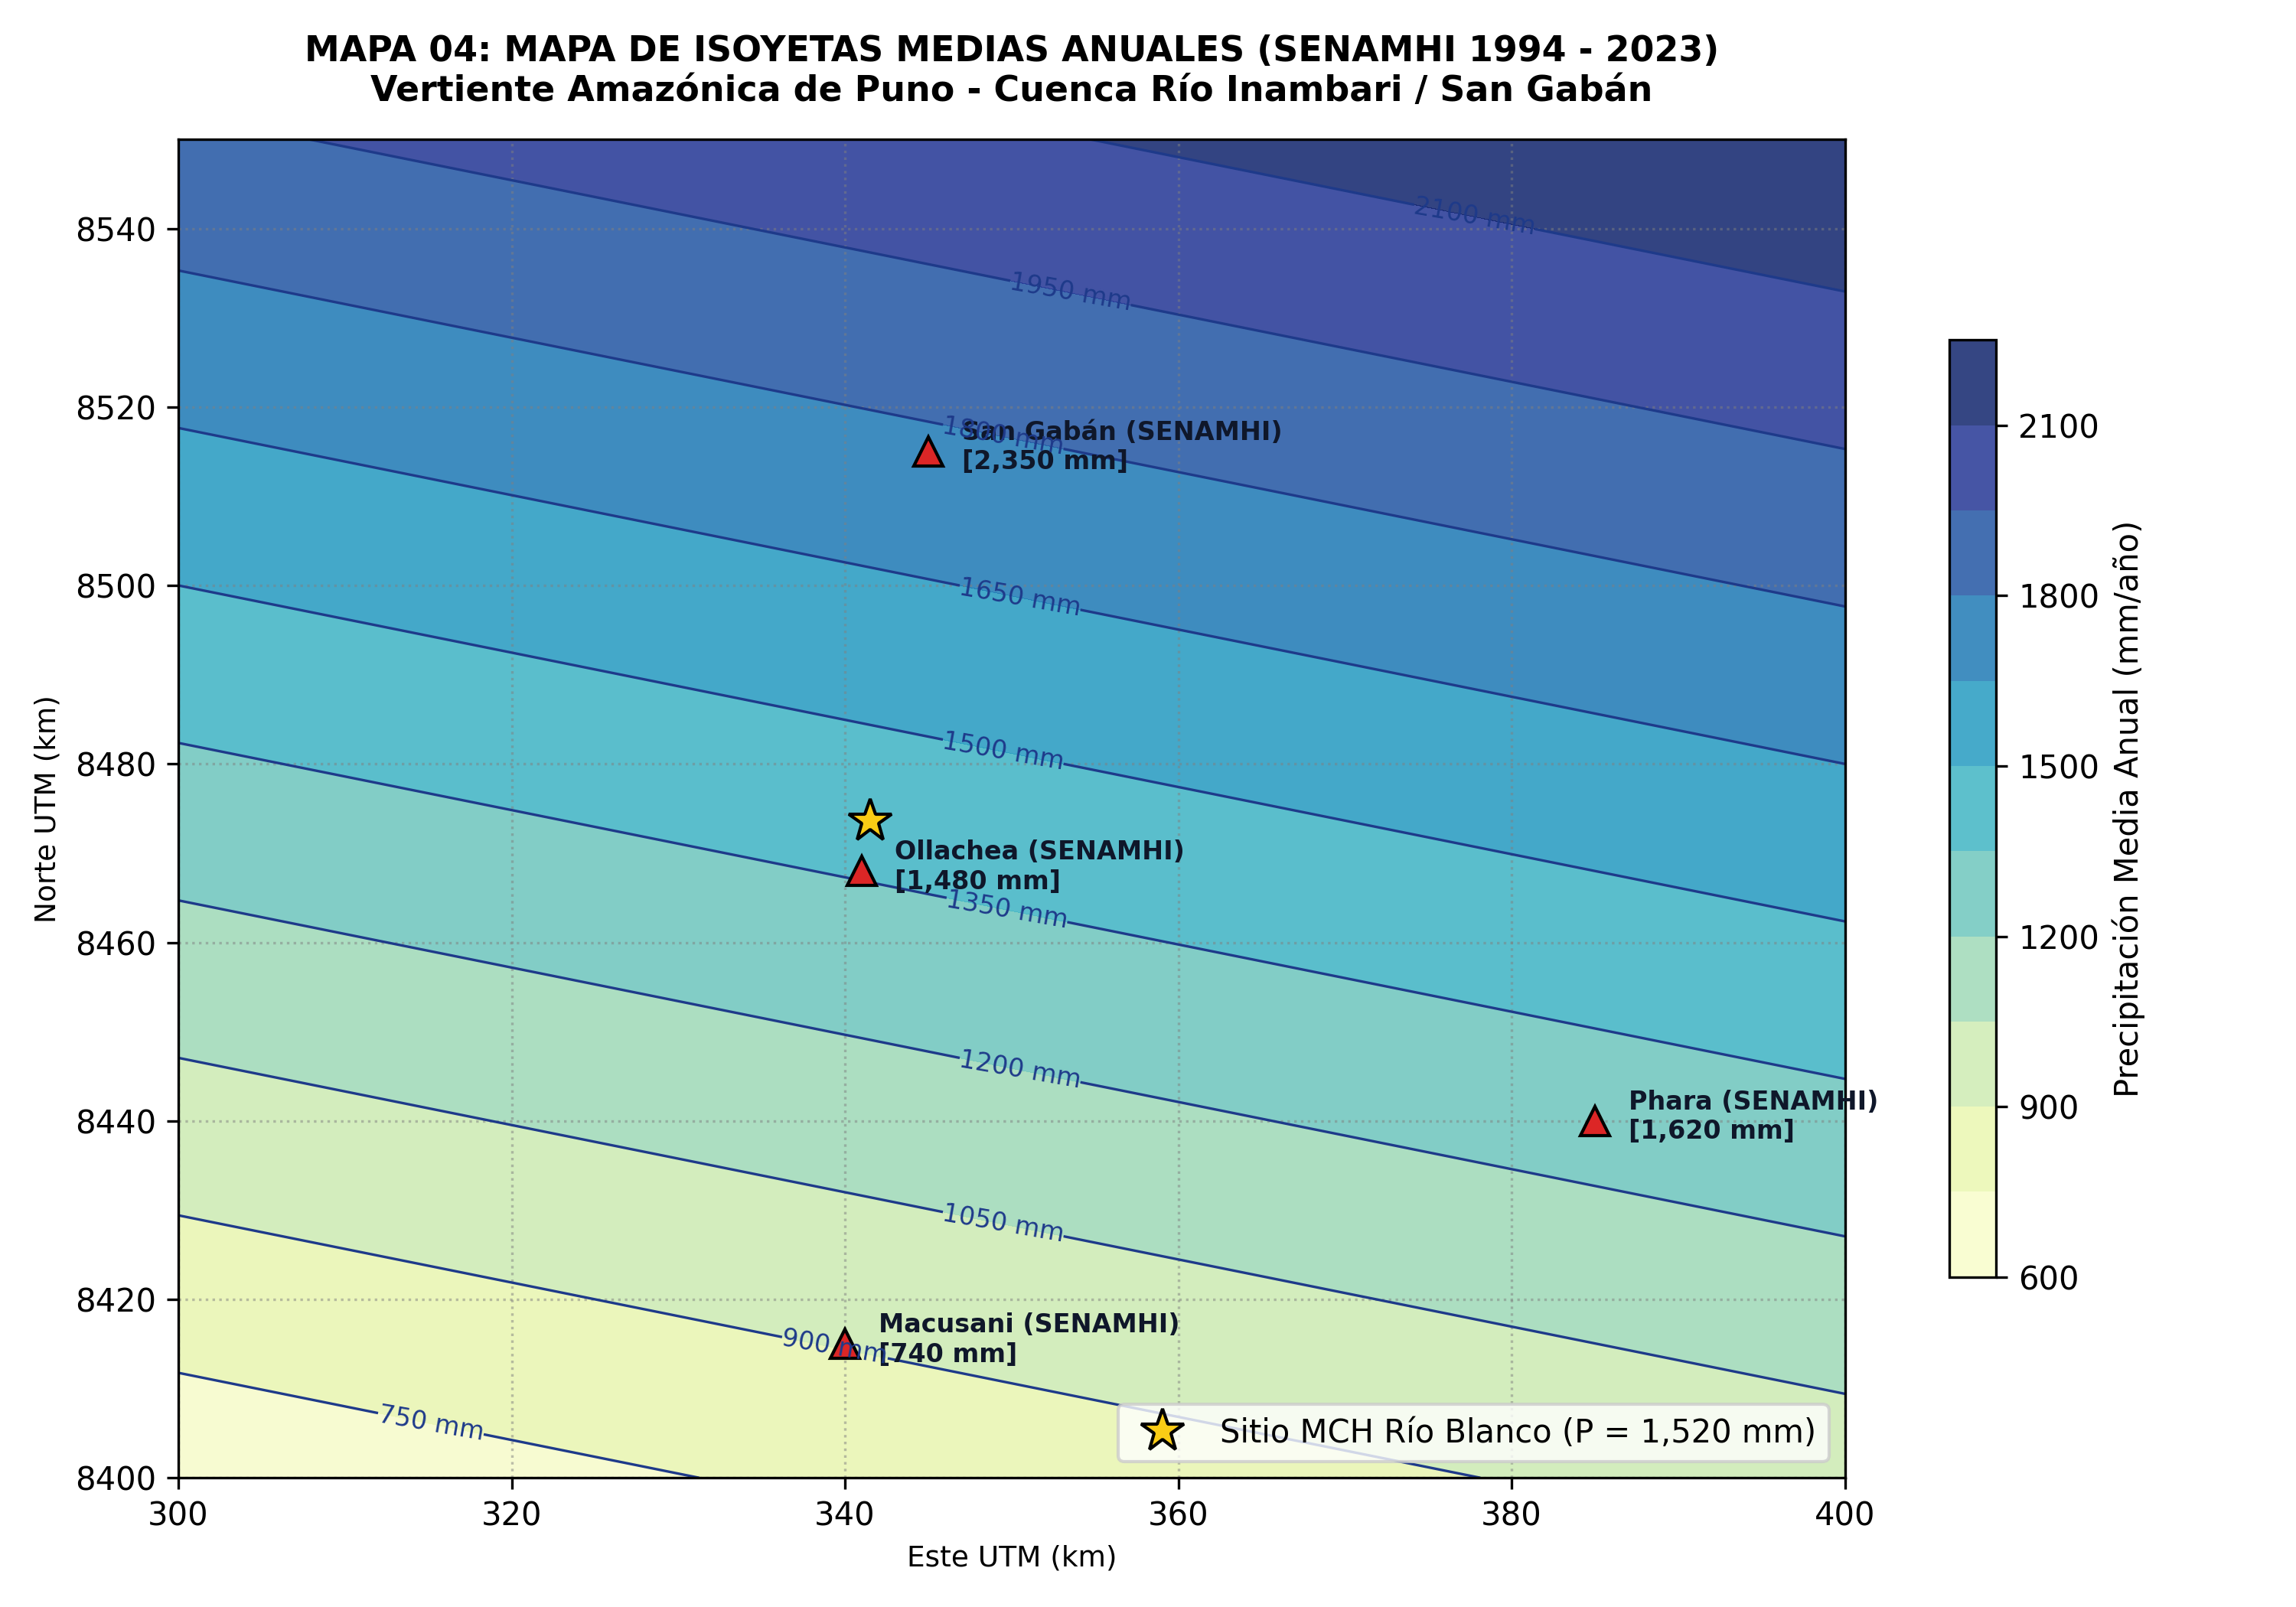
\includegraphics[width=\linewidth]{Mapa_04_Isoyetas_Precipitacion_Senamhi.png}
\caption{LÁMINA LAM-04: Distribución Espacial de Isoyetas de Precipitación SENAMHI (1994-2023).}
\end{figure}

\begin{figure}[H]
\centering
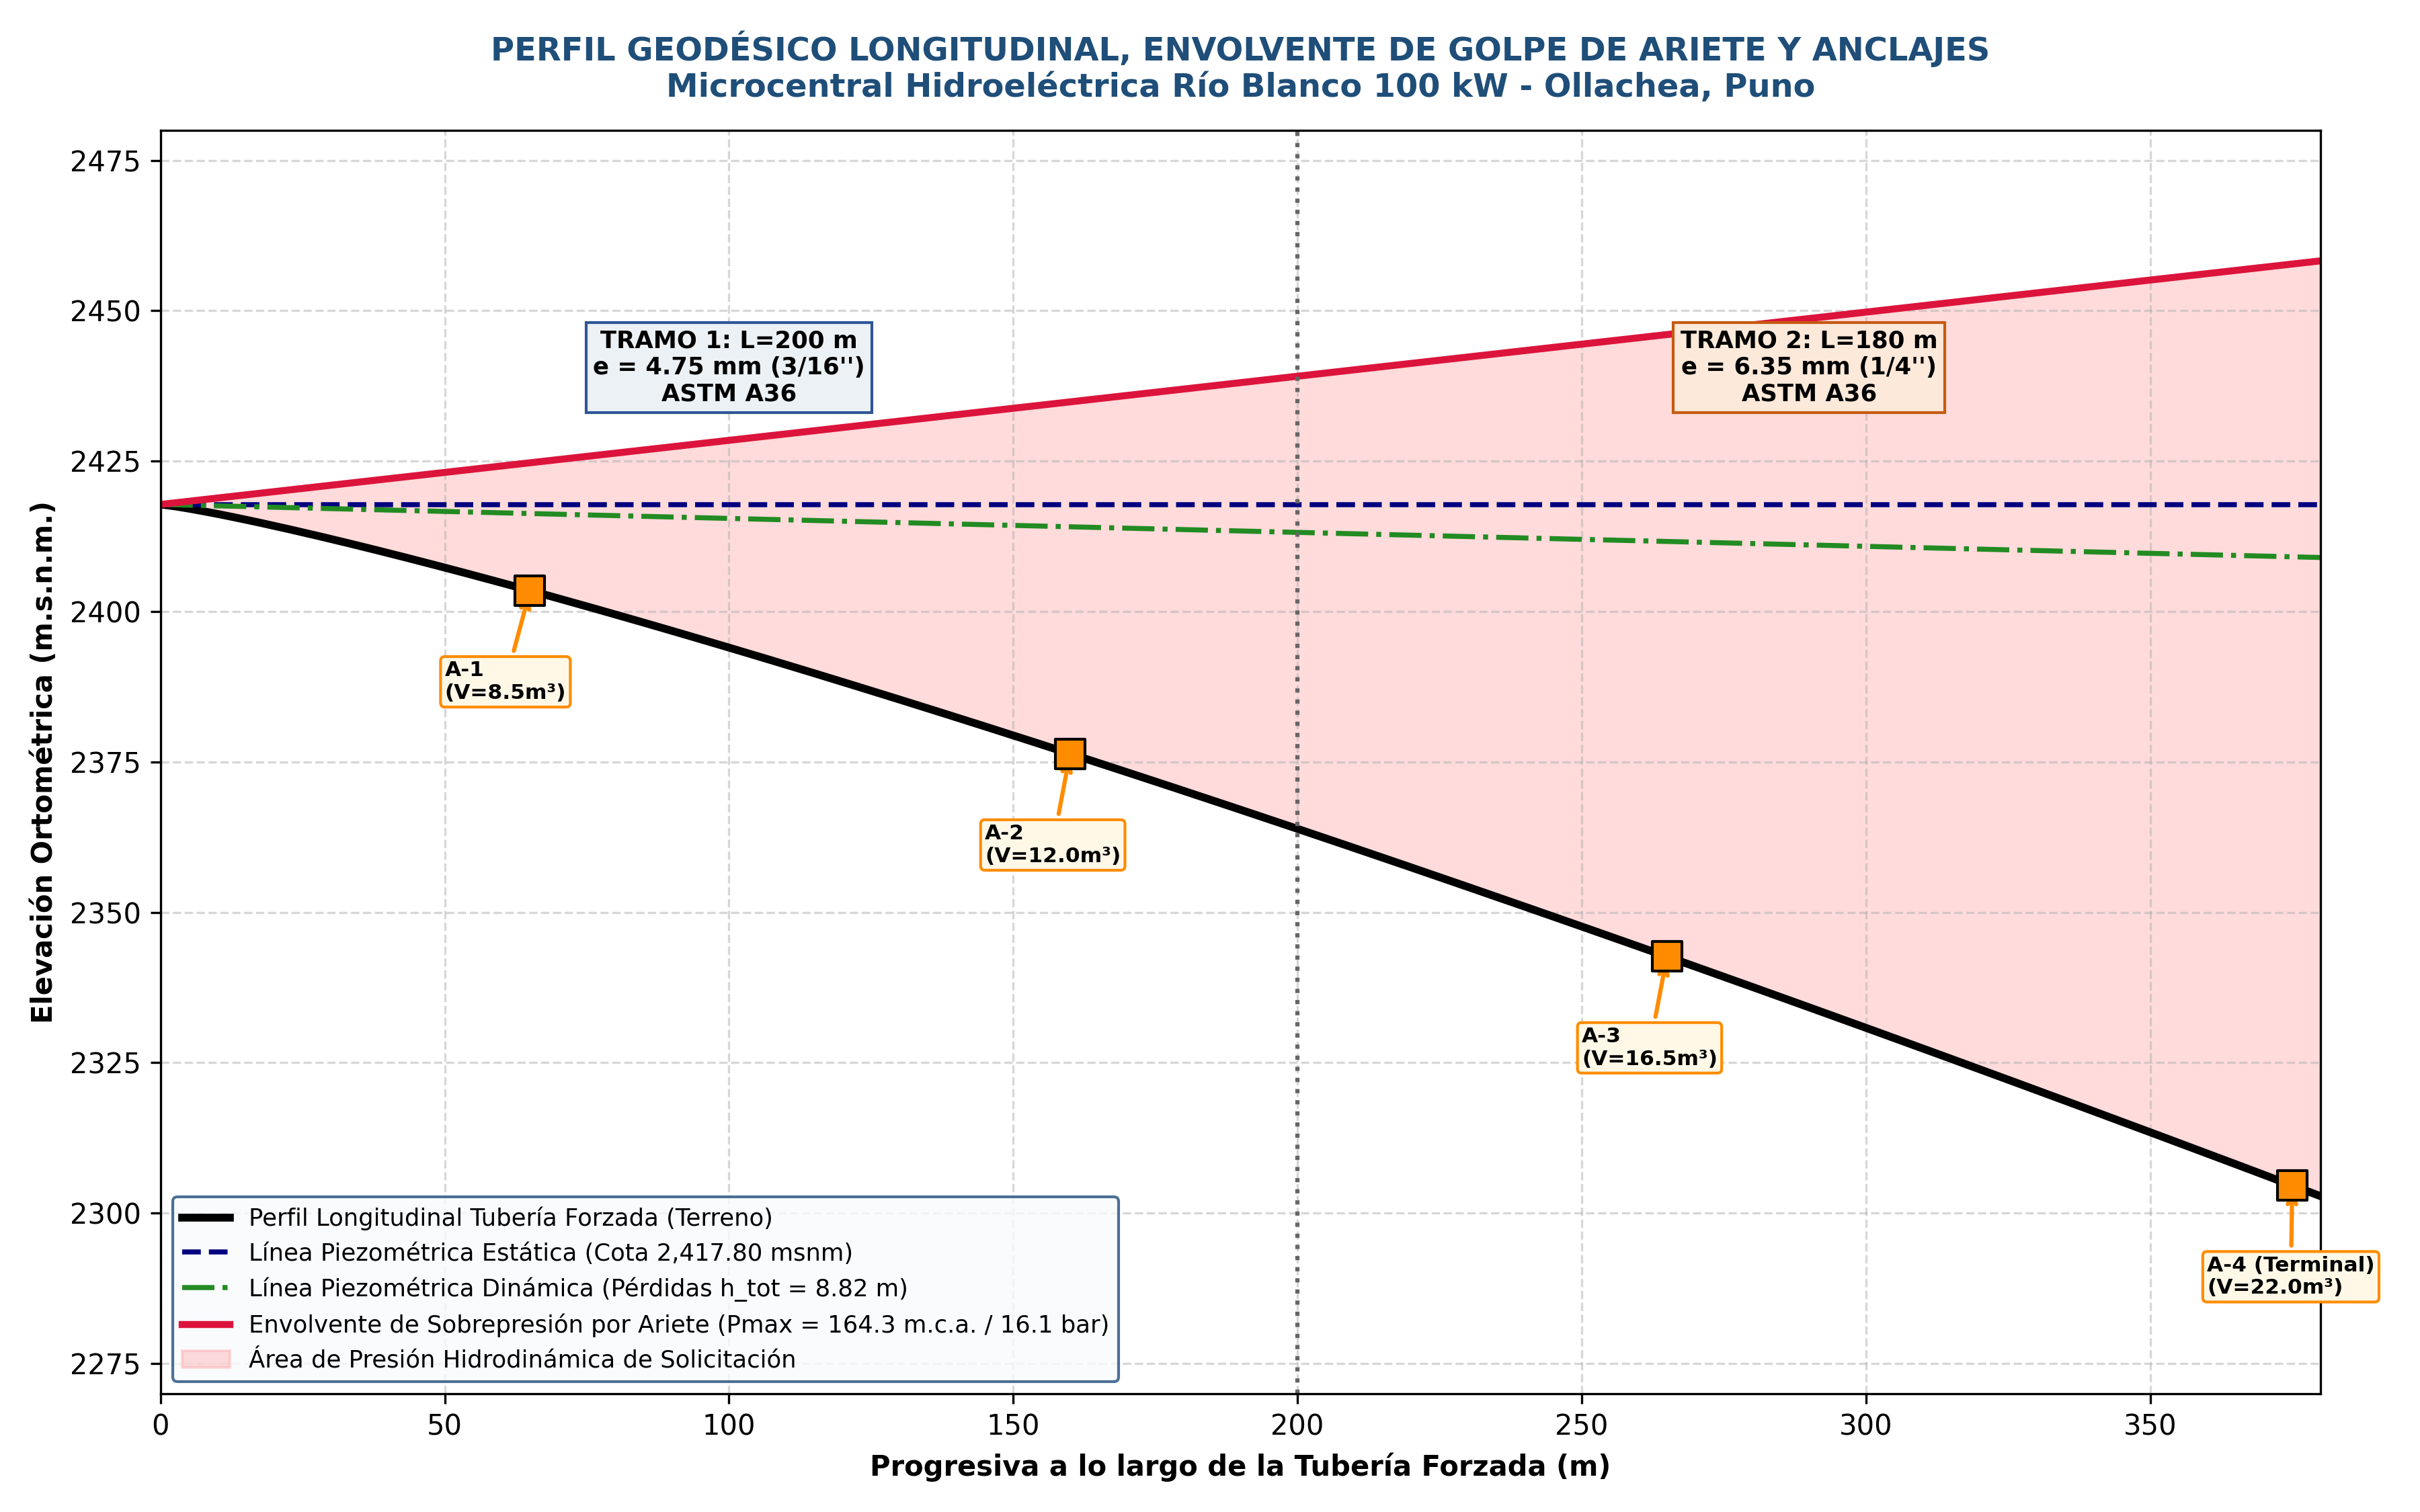
\includegraphics[width=\linewidth]{Mapa_05_Perfil_Longitudinal_Tuberia_Forzada.png}
\caption{LÁMINA LAM-05: Perfil Geodésico Longitudinal, Envolvente de Golpe de Ariete y Bloques de Anclaje.}
\end{figure}

\begin{figure}[H]
\centering
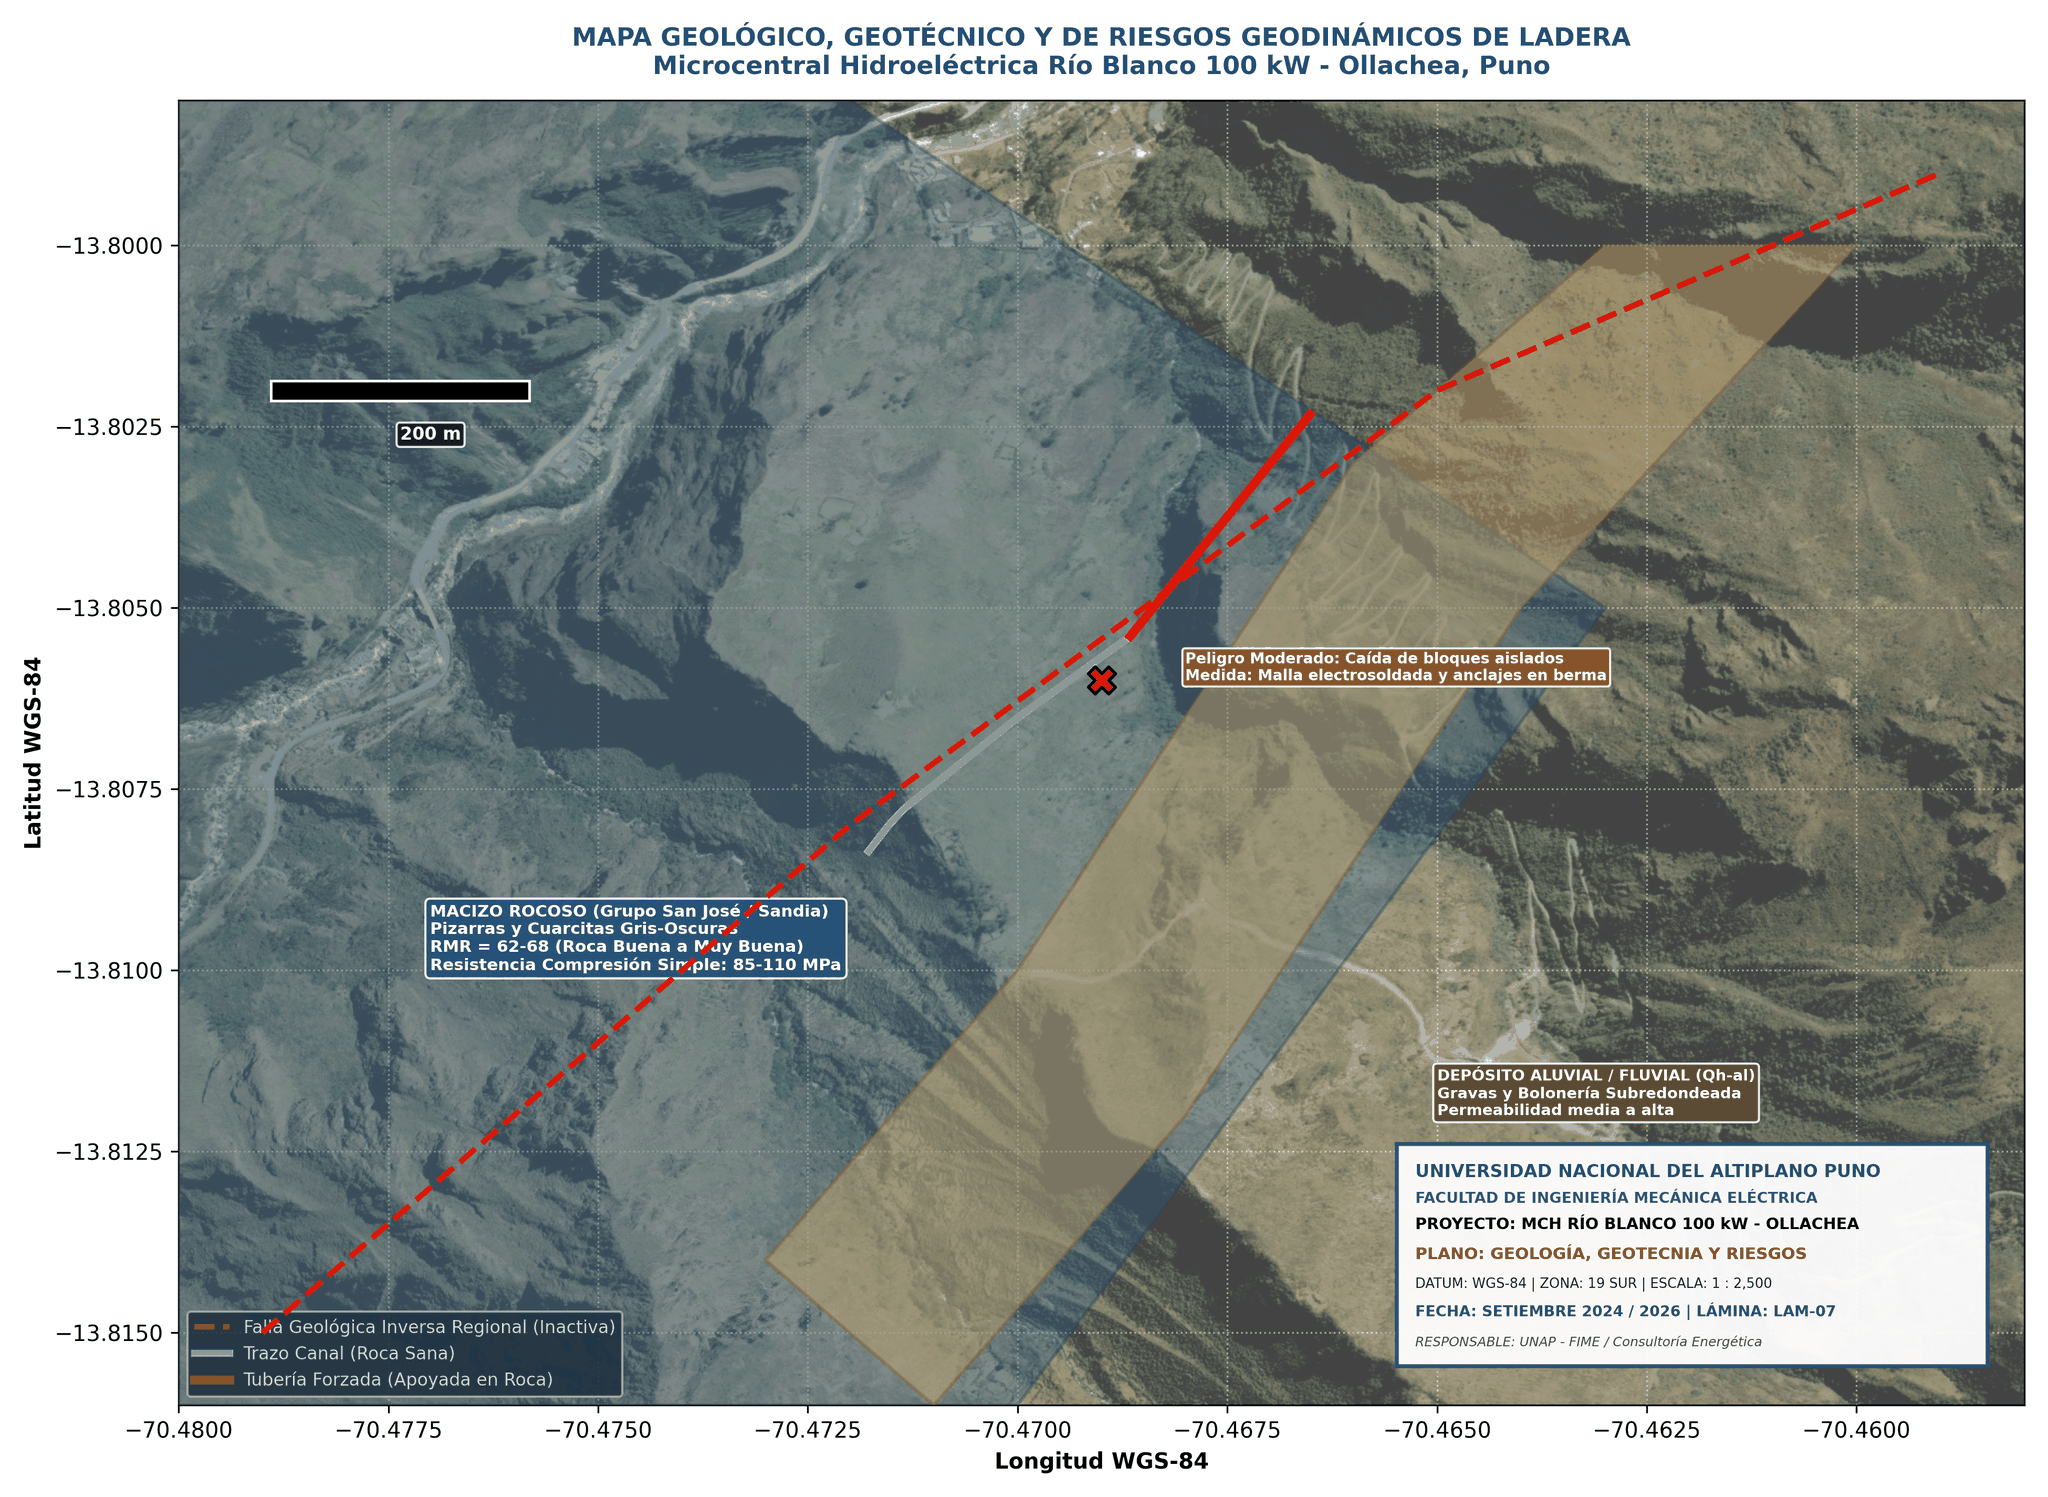
\includegraphics[width=\linewidth]{Mapa_07_Geologico_Geotecnico_Laderas.png}
\caption{LÁMINA LAM-07: Mapa Geológico, Geotécnico y Zonificación de Riesgos de Ladera.}
\end{figure}

\begin{figure}[H]
\centering
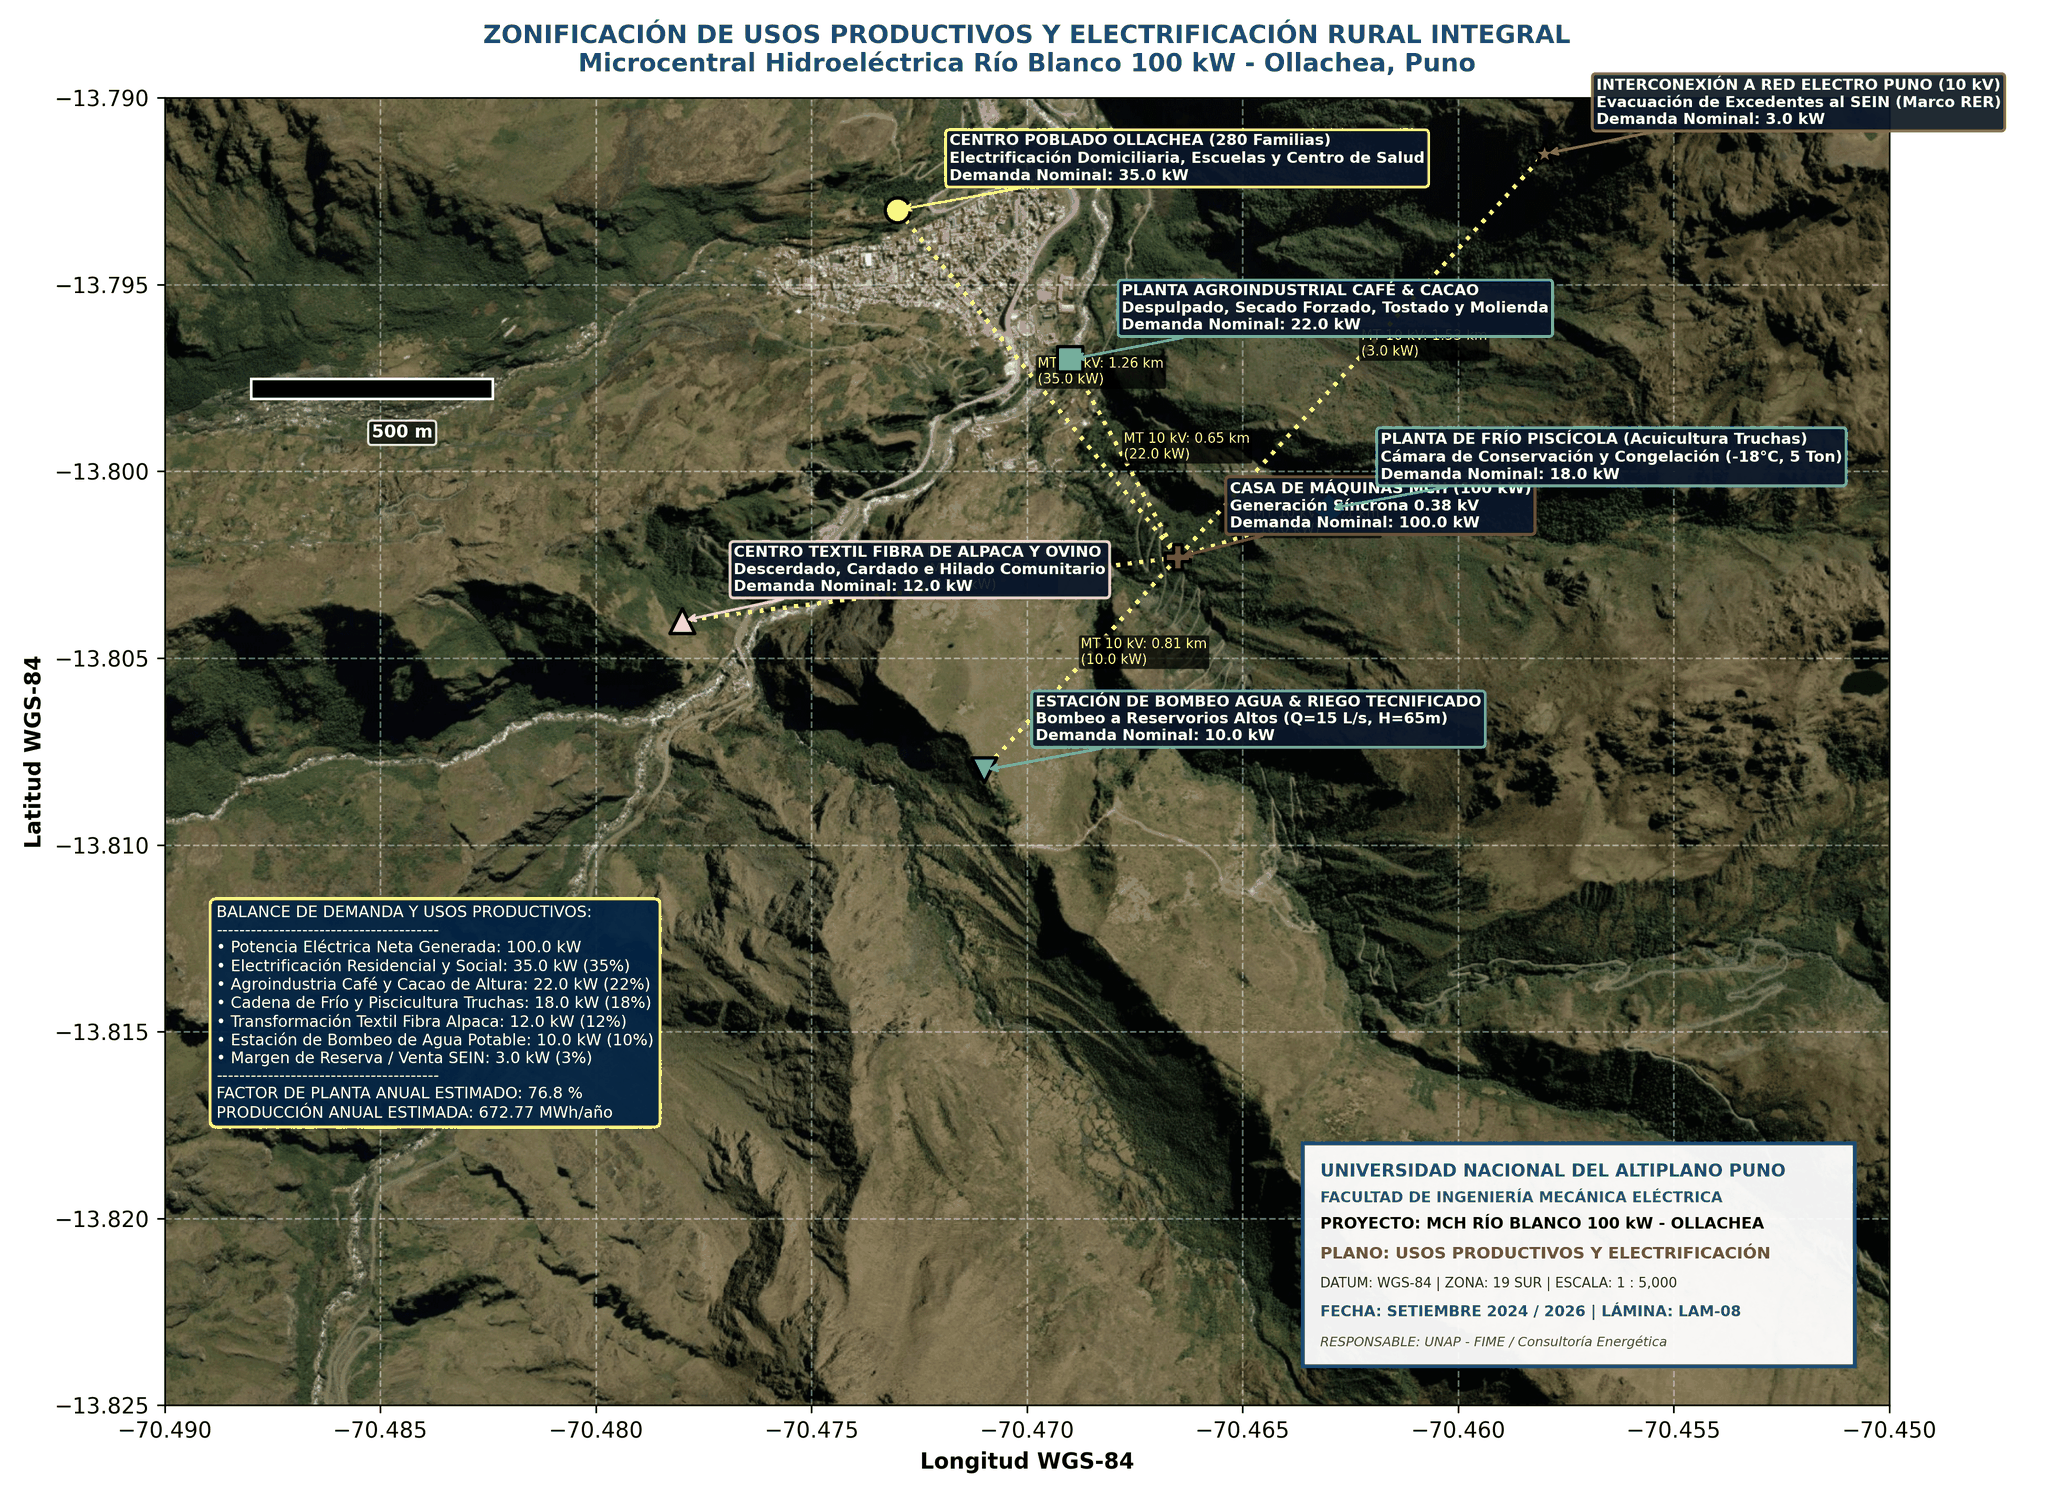
\includegraphics[width=\linewidth]{Mapa_08_Zonificacion_Usos_Productivos_Electrificacion.png}
\caption{LÁMINA LAM-08: Zonificación de Usos Productivos y Electrificación Rural Integral.}
\end{figure}

\chapter{Planos Técnicos de Ingeniería de Detalle}

\begin{figure}[H]
\centering
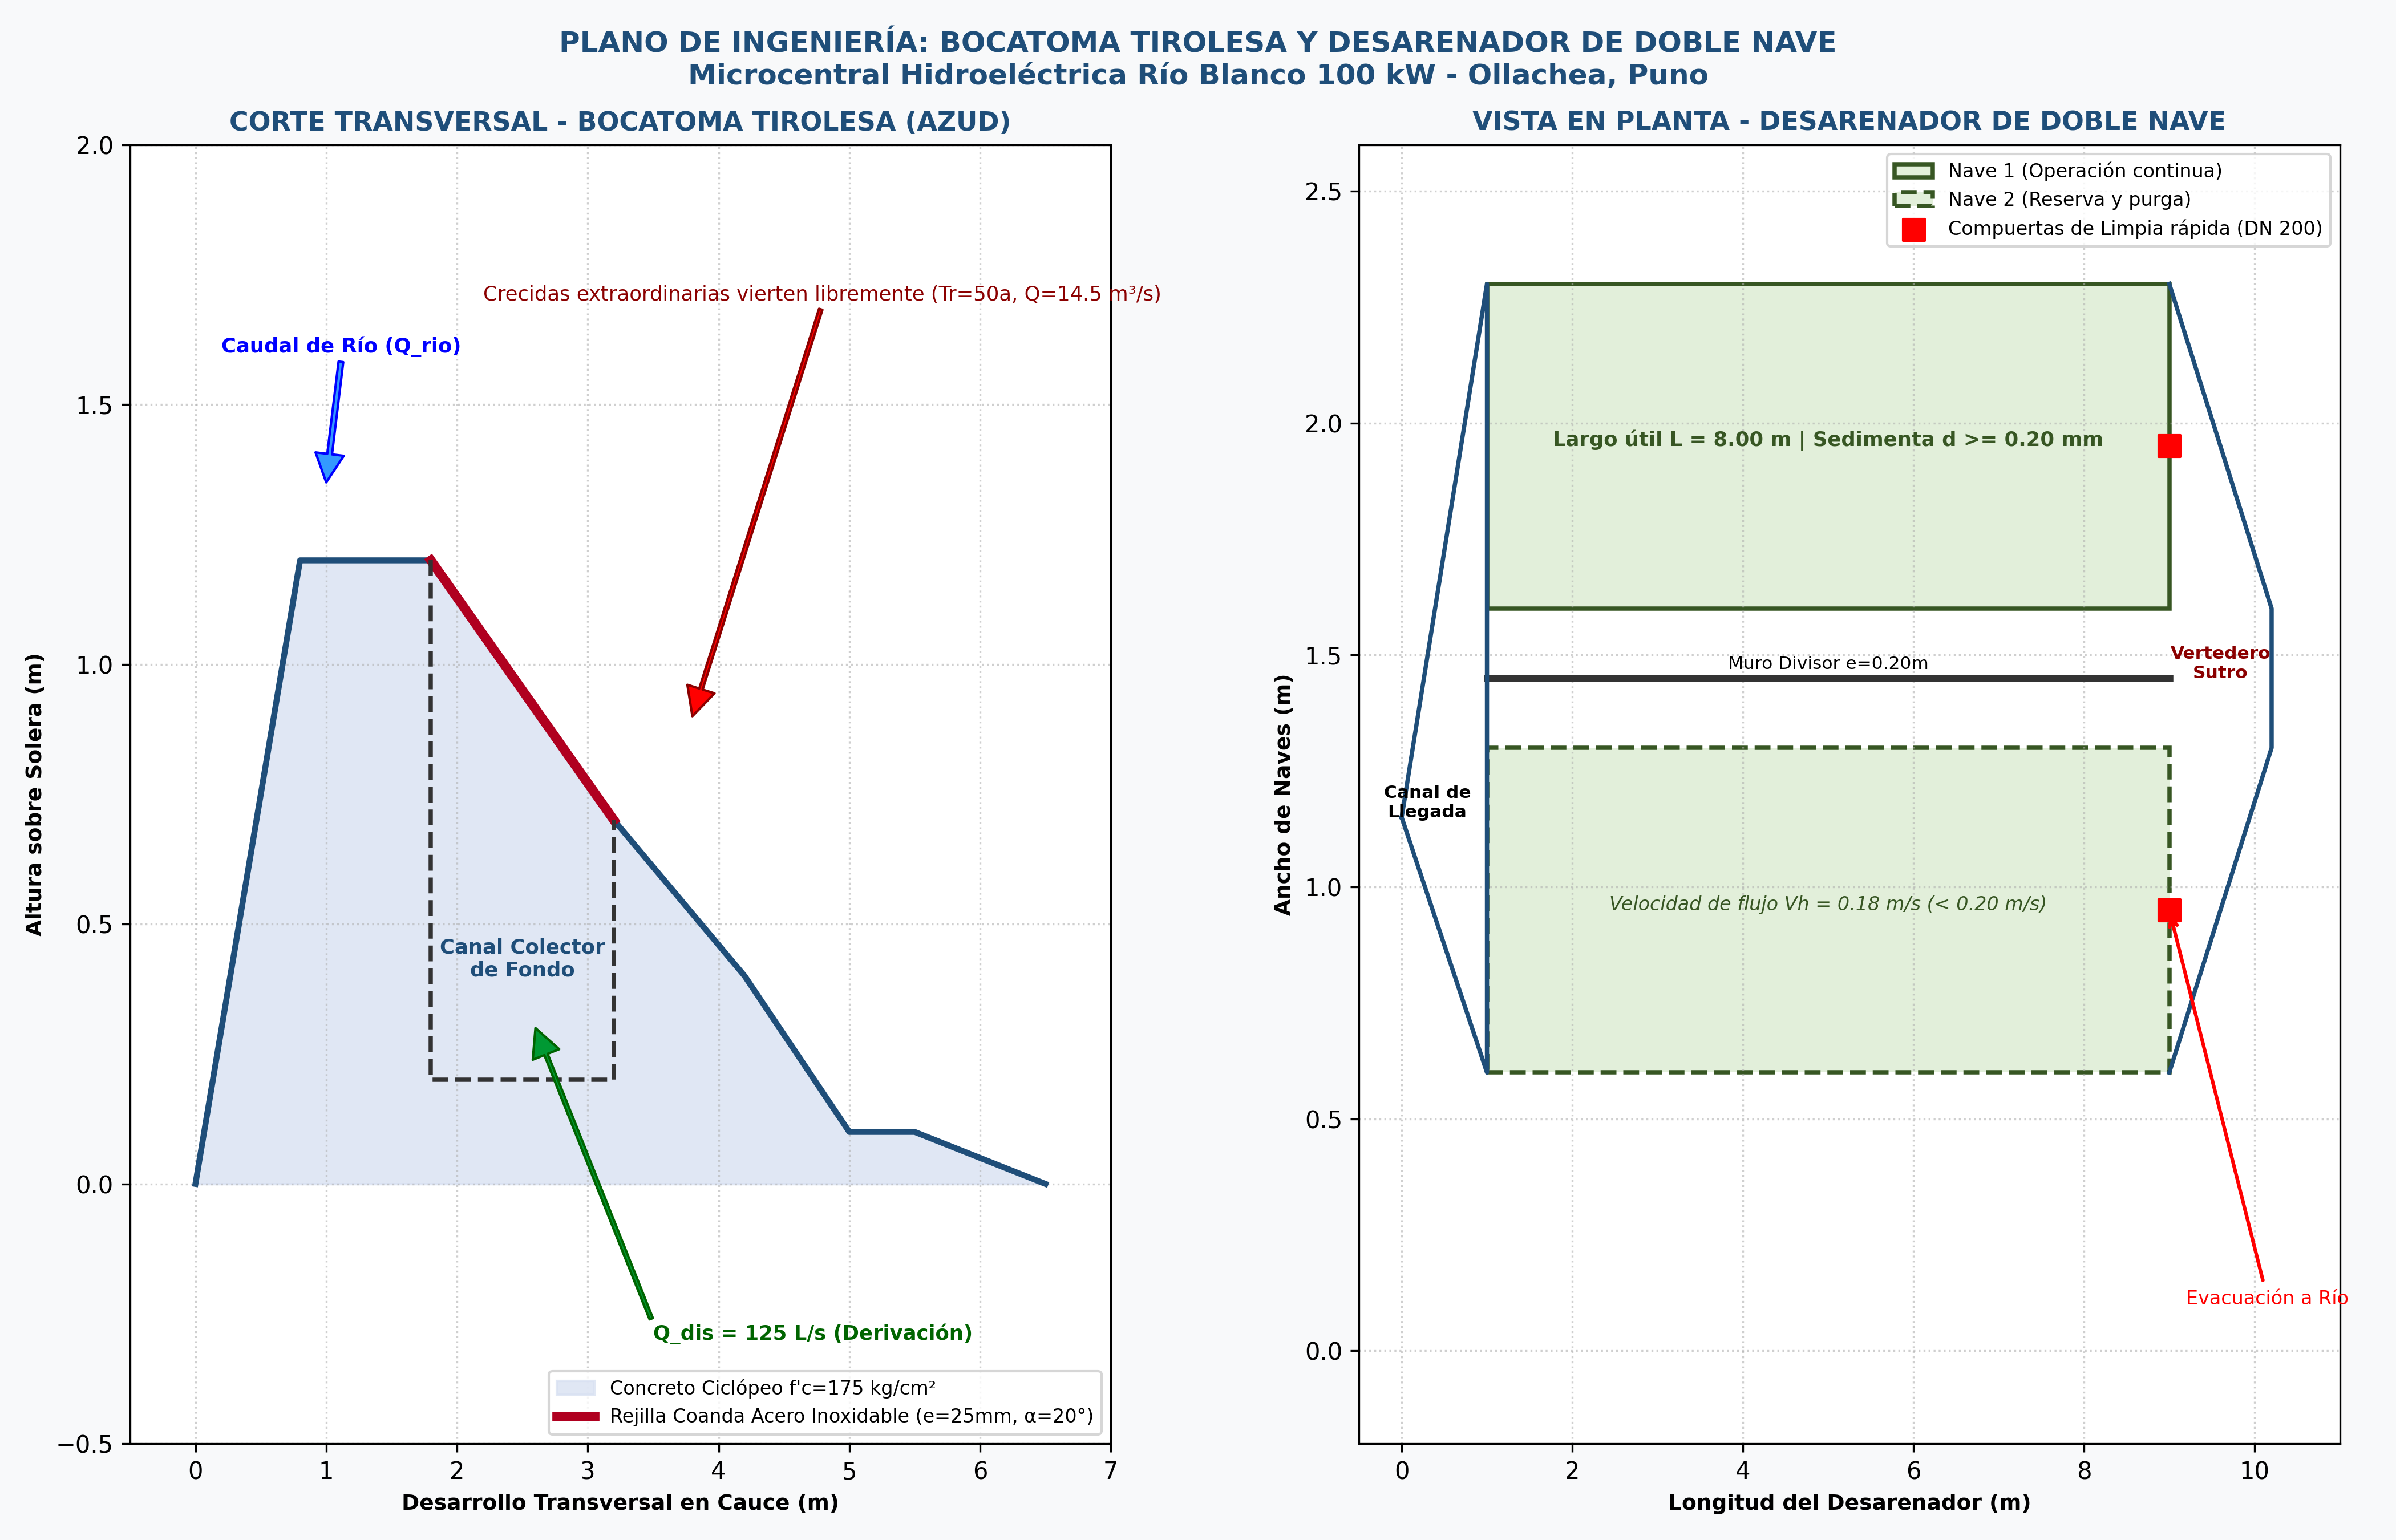
\includegraphics[width=\linewidth]{Plano_01_Bocatoma_Tirolesa_Desarenador.png}
\caption{PLANO PL-01: Bocatoma Tirolesa con Azud y Desarenador de Doble Nave.}
\end{figure}

\begin{figure}[H]
\centering
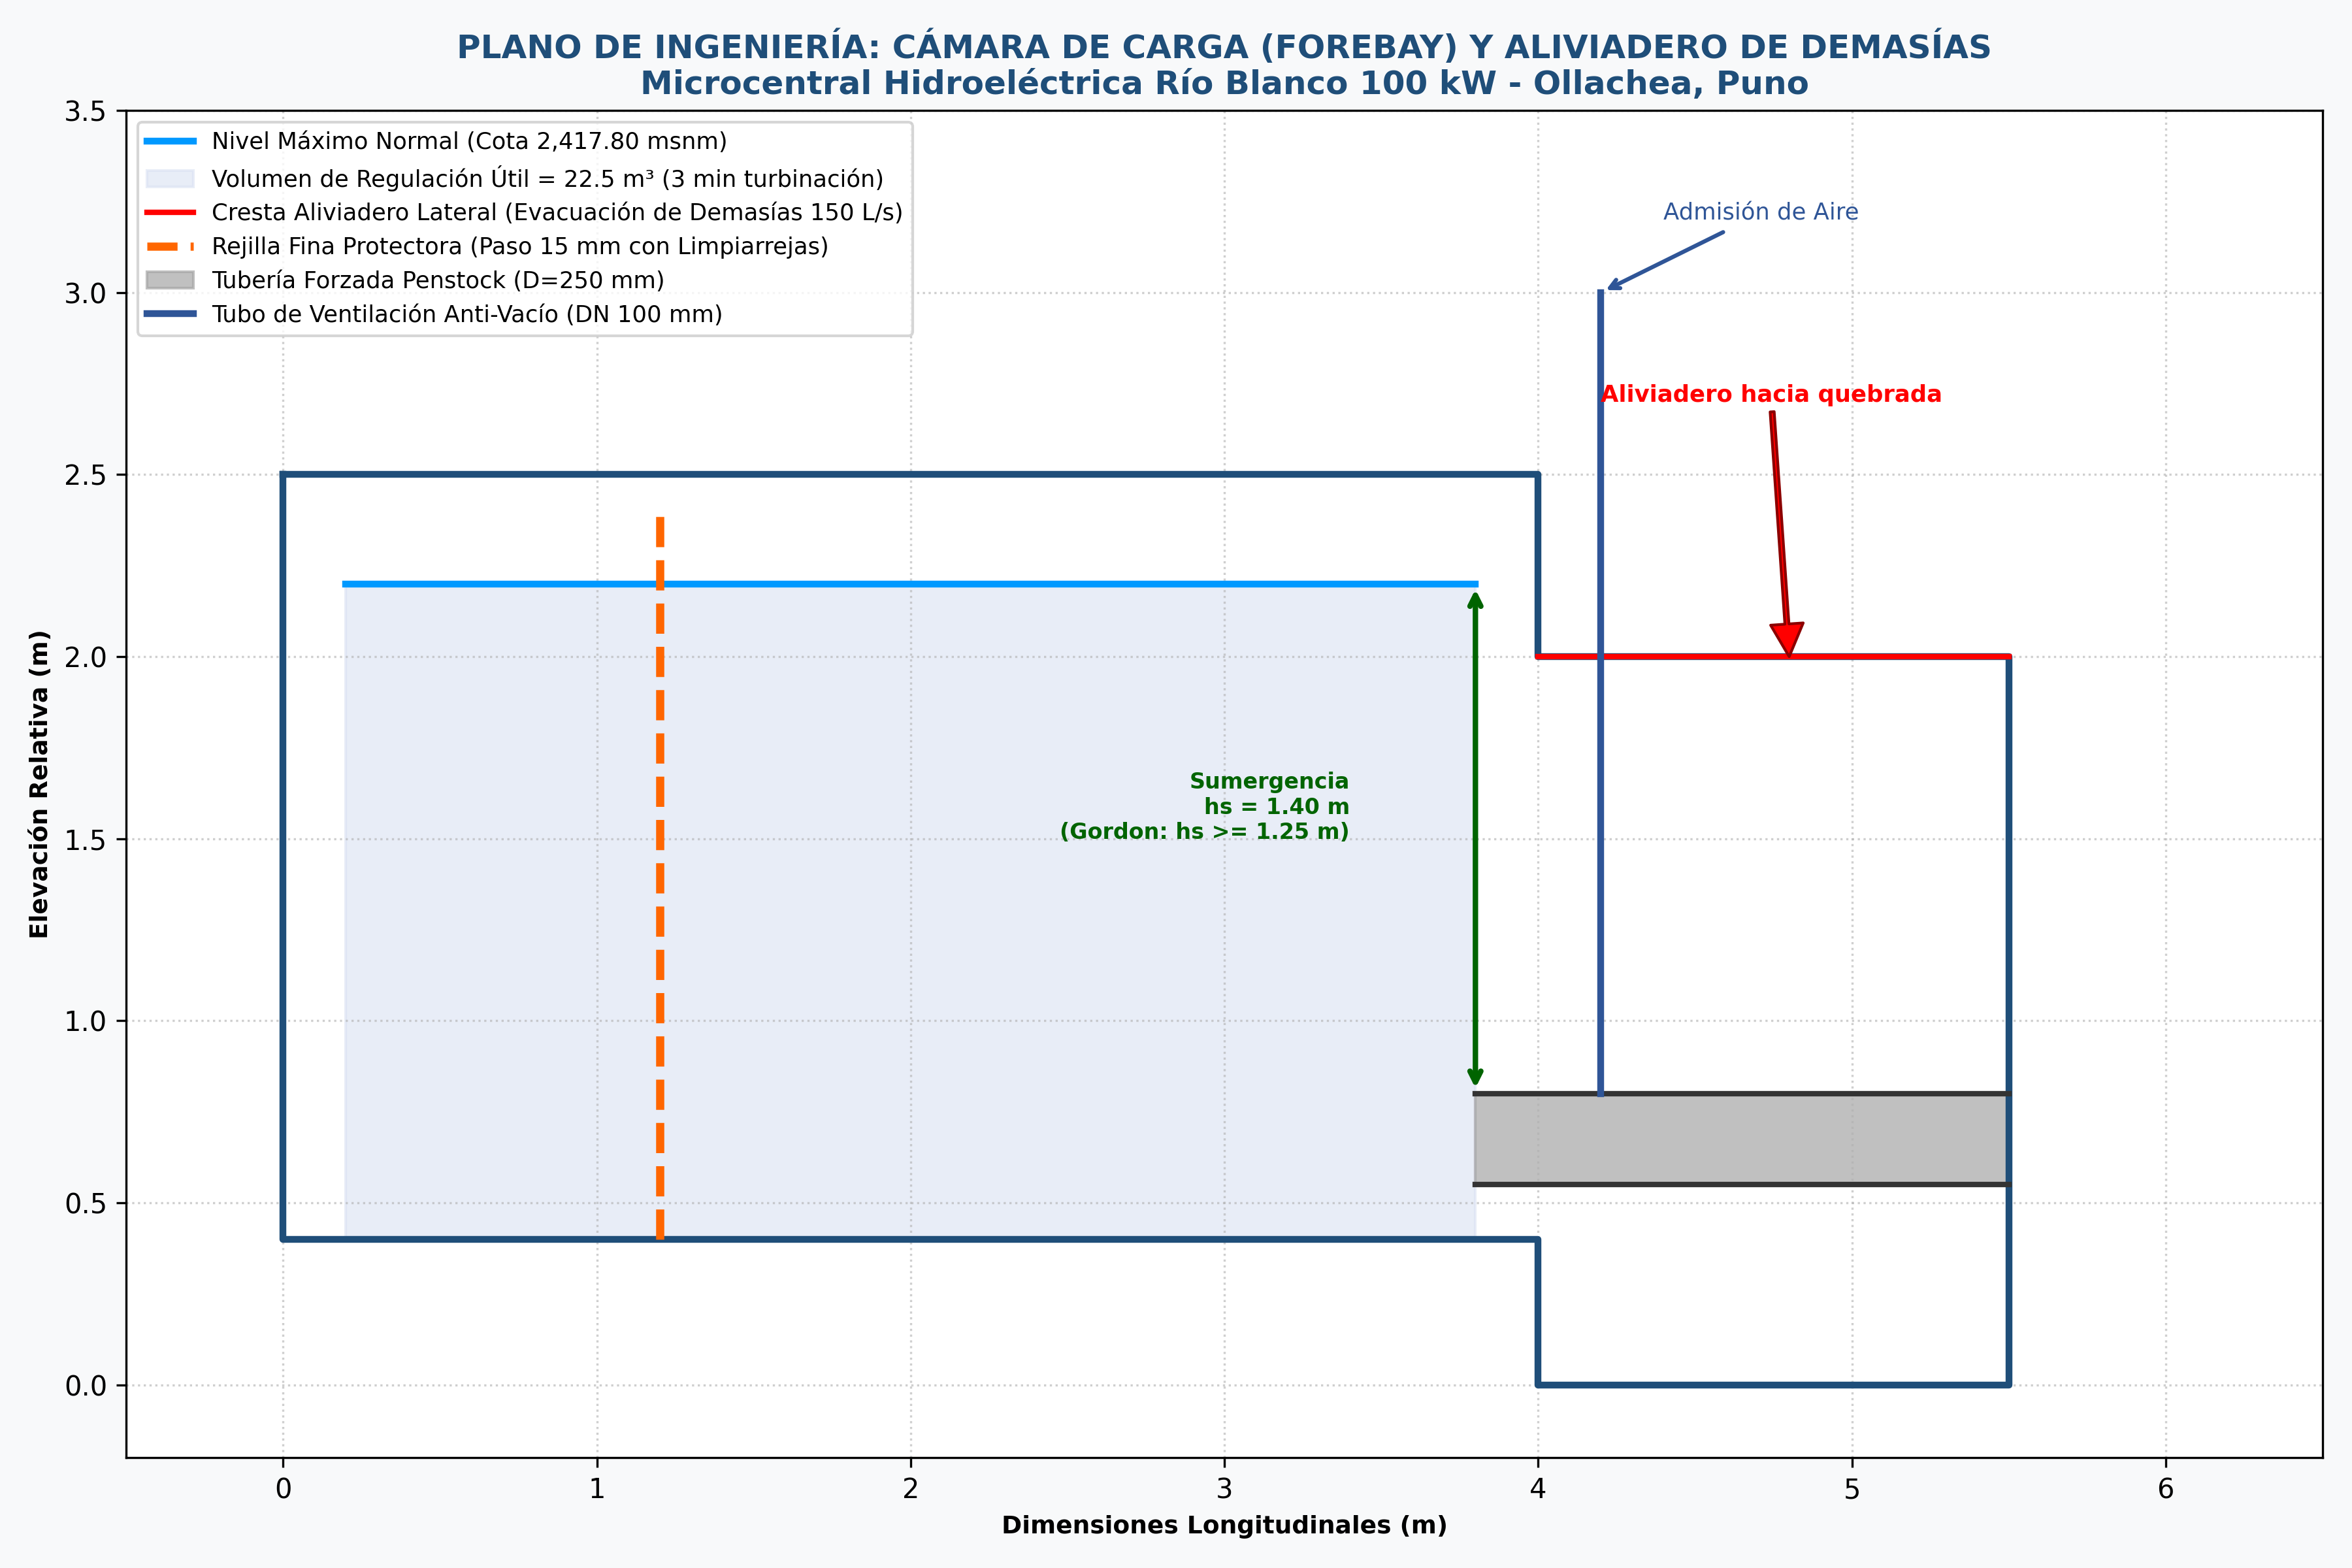
\includegraphics[width=\linewidth]{Plano_02_Camara_Carga_Aliviadero.png}
\caption{PLANO PL-02: Cámara de Carga (Forebay) y Aliviadero Lateral de Demasías.}
\end{figure}

\begin{figure}[H]
\centering
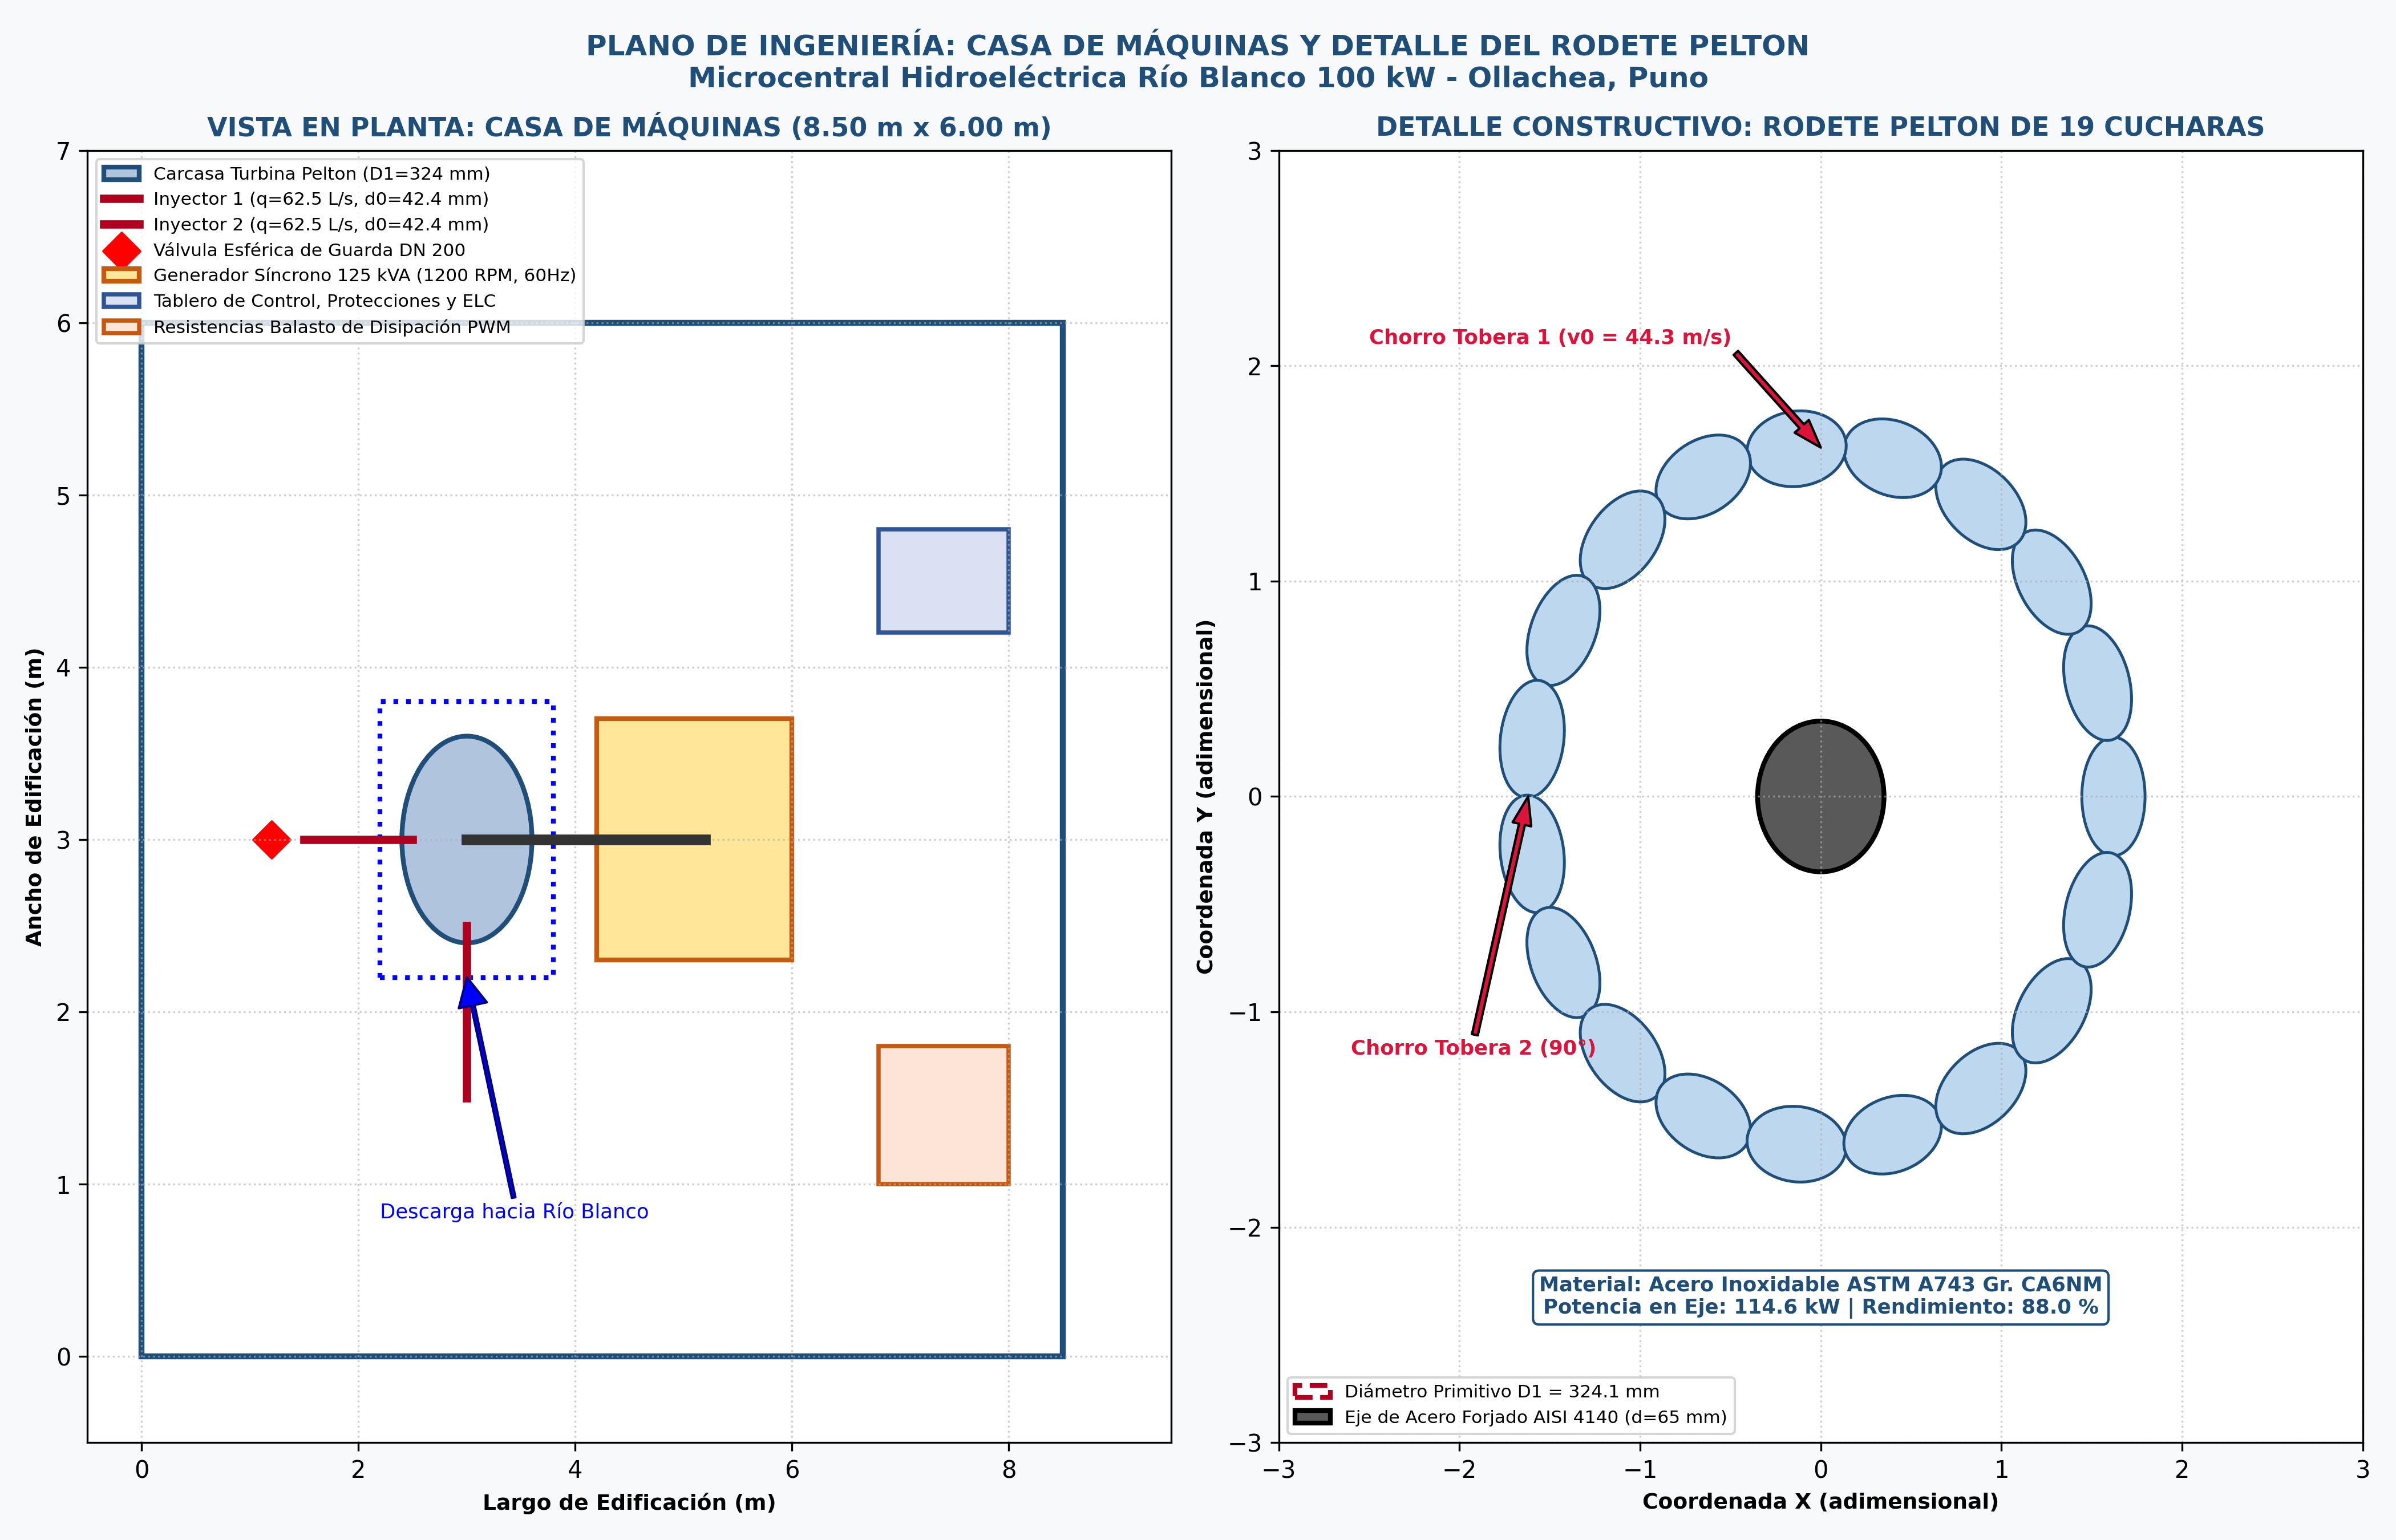
\includegraphics[width=\linewidth]{Plano_03_Casa_Maquinas_Grupo_Pelton.png}
\caption{PLANO PL-03: Disposición General de Casa de Máquinas y Geometría del Rodete Pelton.}
\end{figure}

\begin{figure}[H]
\centering
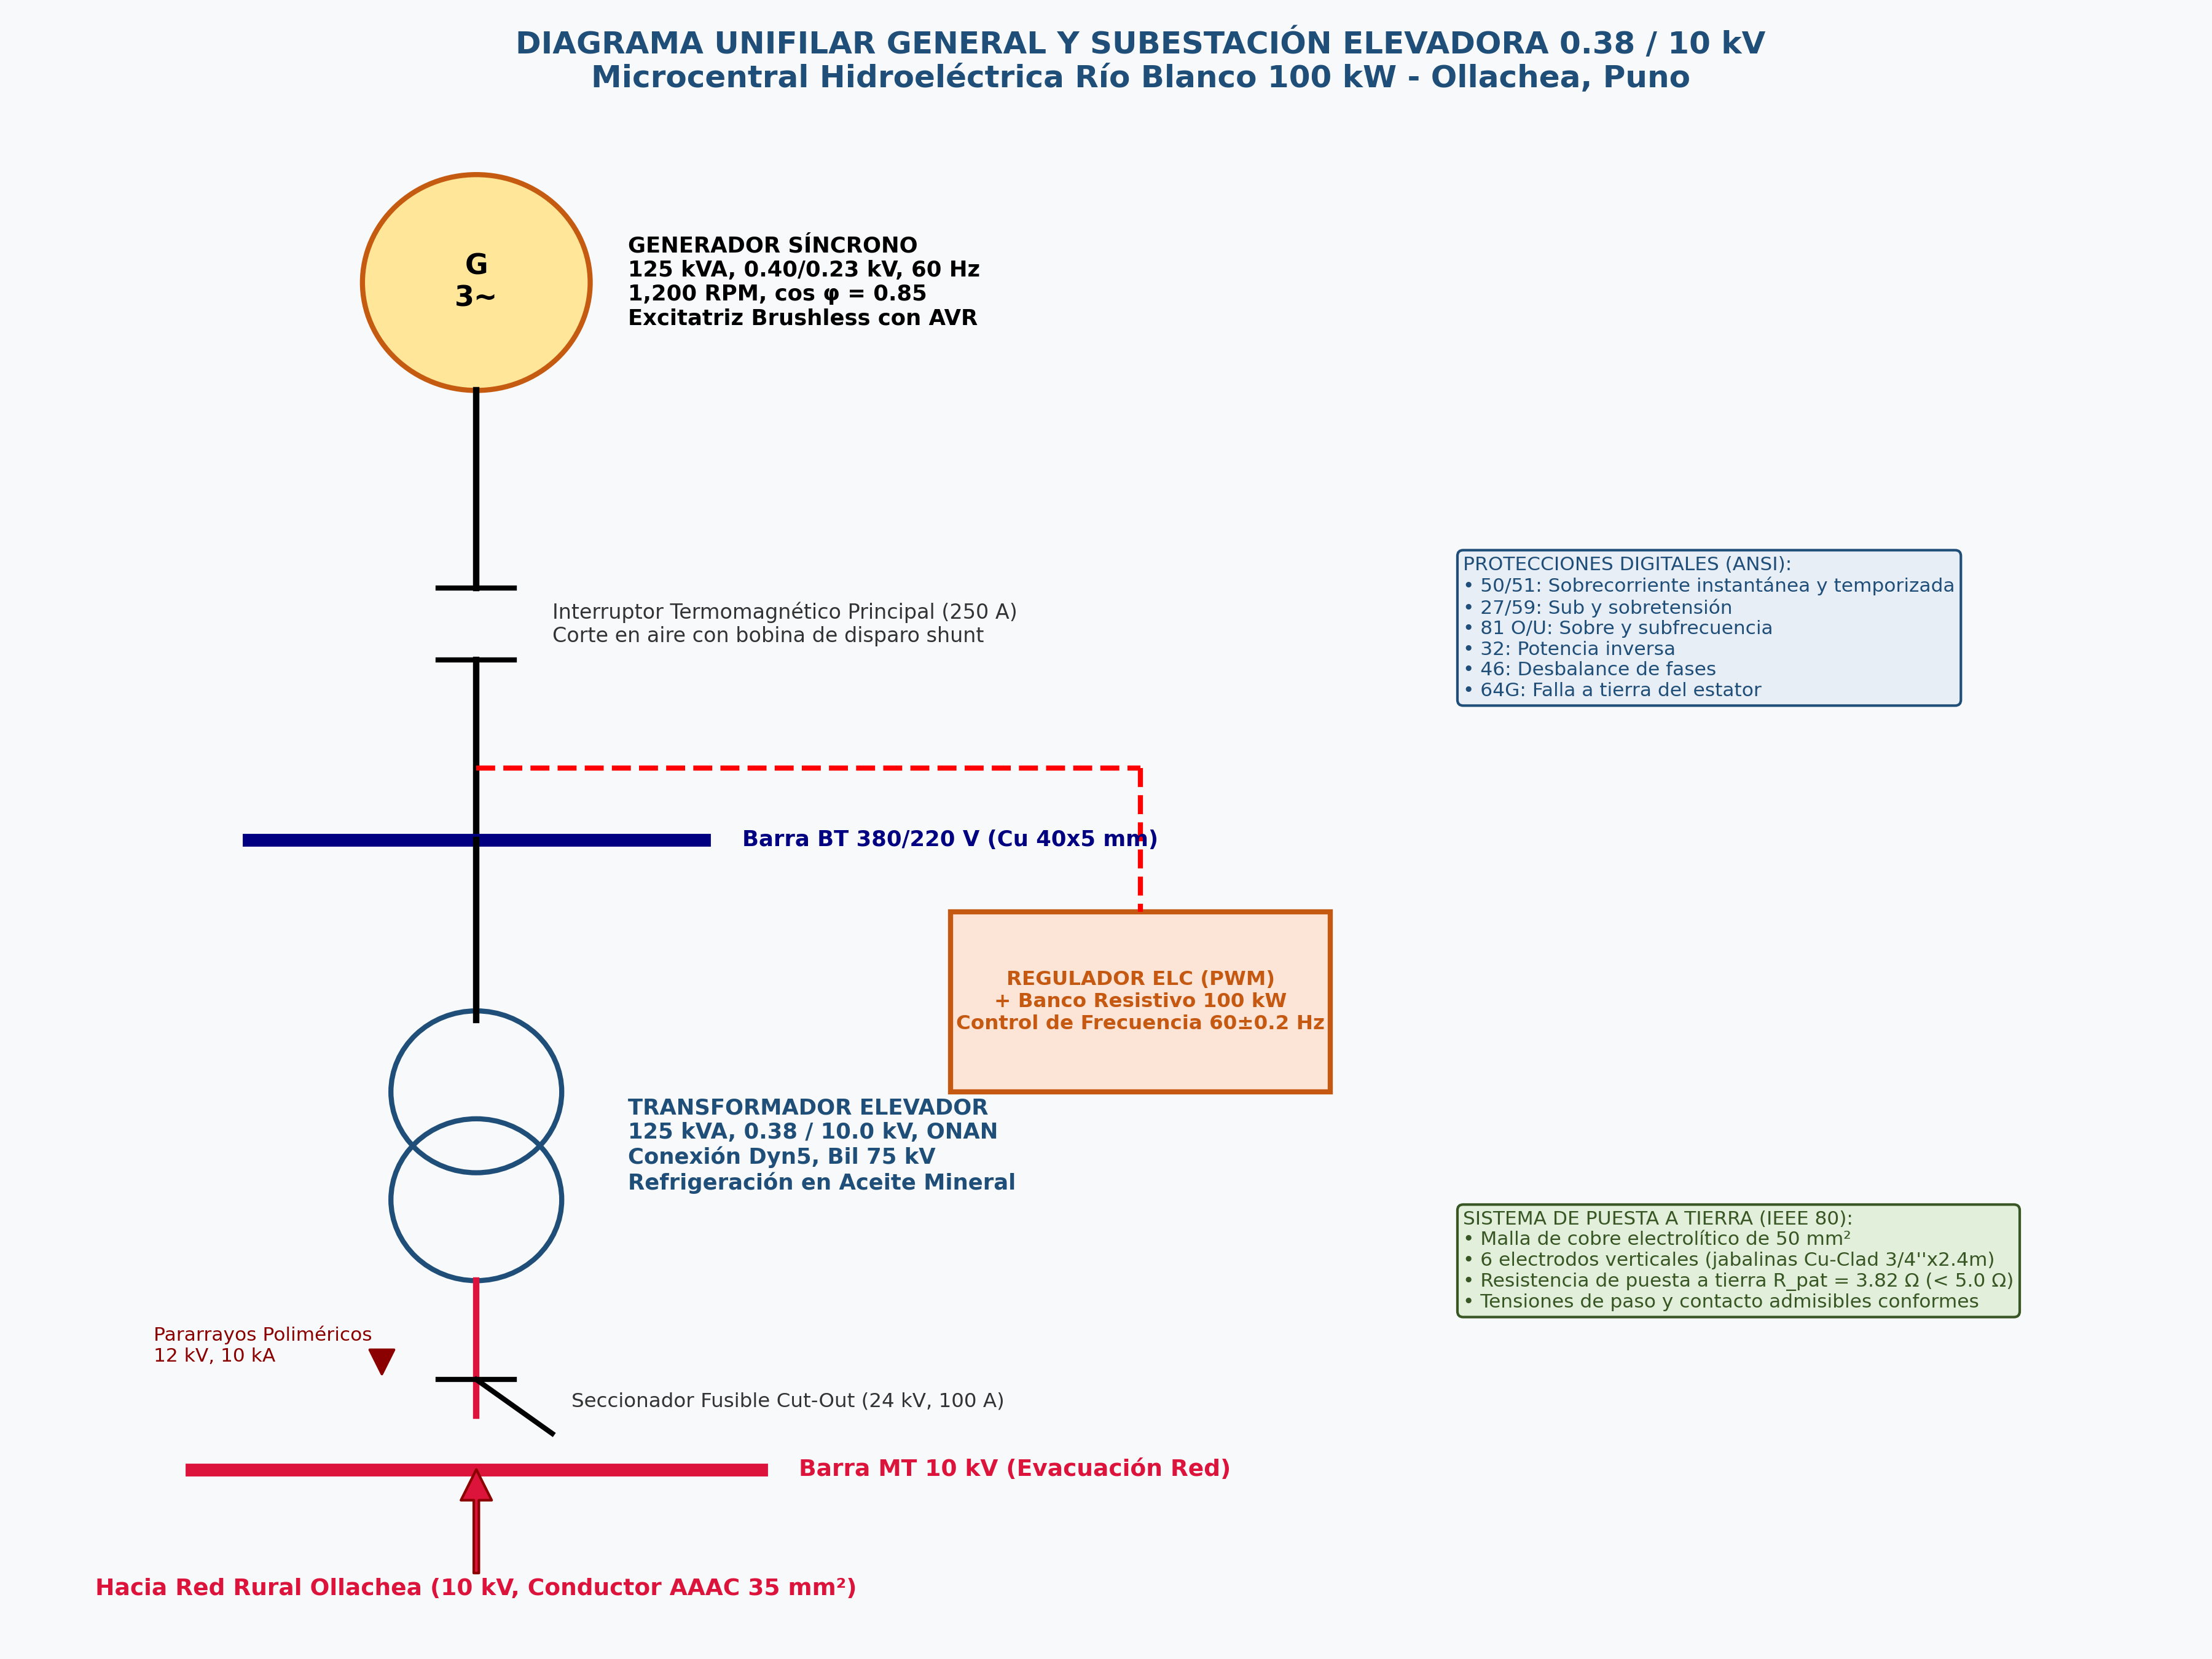
\includegraphics[width=\linewidth]{Plano_04_Diagrama_Unifilar_Subestacion.png}
\caption{PLANO PL-04: Diagrama Unifilar General, Subestación Elevadora 0.38/10 kV y Malla a Tierra.}
\end{figure}

\end{document}
